\documentclass[10pt,a4paper]{scrartcl}

% Language setting
% Replace `english' with e.g. `spanish' to change the document language
\usepackage[english]{babel}
\usepackage{float}
%\usepackage{subfloat}

% Set page size and margins
% Replace `letterpaper' with `a4paper' for UK/EU standard size
\usepackage[letterpaper,top=2cm,bottom=2cm,left=3cm,right=3cm,marginparwidth=1.75cm]{geometry}

% Useful packages
\usepackage{amsmath}
\usepackage{amssymb} %collection de symboles mathématiques
\usepackage{amsfonts}
\usepackage{physics}
\usepackage{graphicx}
\usepackage{caption}
\usepackage{subcaption}
\usepackage[colorlinks=true, allcolors=blue]{hyperref}

\usepackage{color} %gestion de diffèrentes couleurs
\usepackage{xcolor}
\definecolor{linkcolor}{rgb}{0,0,0.6} %définition de la couleur des liens pdf
%\usepackage[pdftex, colorlinks=true, pdfstartview=FitV, linkcolor=linkcolor, citecolor=linkcolor, urlcolor=linkcolor, hyperindex=true, hyperfigures=false]{hyperref} % fichiers pdf 'intelligents', avec des liens entre les références, etc.
%\usepackage[colorlinks=true, allcolors=blue]{hyperref}




%\usepackage{gensymb}
\usepackage[T1]{fontenc} %codage moderne des caractères sous Latex
\usepackage[utf8]{inputenc} %utilisation directe des caractères accentués sur pc

\usepackage[babel=true]{csquotes}
\usepackage{xspace}


\usepackage{sistyle} %mise en forme des unités




\usepackage{fancyhdr} %entêtes et pieds de pages personnalisés
\usepackage{array}
\usepackage{multicol}
\usepackage{enumitem}
\usepackage{mathenv}


\usepackage{ulem}
\usepackage{authblk} %for affiliations

\title{tRNA gene set evolution}
%
\author[1]{Miguel Pedraza}
\affil[1]{Aix-Marseille Université, France}
%
%
%
%\date{}
%
%
%
\usepackage{setspace}
\usepackage[displaymath, mathlines]{lineno}
\onehalfspacing
%\linenumbers
\def\linenumberfont{\normalfont\footnotesize\sffamily}

\begin{document}


\maketitle
\tableofcontents
\newpage
%\maketitle



\section{Introduction}

tRNAs are the RNA molecules that are responsible for establishing the link between mRNA and the amino acid sequence of proteins during translation. They bring the amino acids to the ribosome, which then pairs the mRNA codon with the end of tRNA at which there is an anti-codon -- the amino-acid being at the other end of its characteristic shape. 
There are 4*4*4 - 3 stop codons = 61 possible tRNAs, all of which would be needed if translation only relied on the canonical Watson-Crick base pairing (A-U;G-C).
However, the genetic code is redundant, as the 61 coding codons only encode 20 different amino acids. Thus, thanks to the weaker "wobbly pairing", mRNA can be translated by many fewer than 61 distinct tRNAs.

In fact, the tRNA gene set varies a lot between organisms. The question of its evolution is of importance.
In order to observe it \textit{in vitro}, it is possible to perform \textit{evolution experiments}, whereby one engineers a bacterial strain (here SBW25) by deleting one of its tRNA genes present in only one copy (here \textit{SerCGA}, thus creating the strain \textit{delSerCGA}). We can subsequently observe how the resulting lineage evolves and adapts to overcome the growth defect induced by the deletion.  Concretely, bacteria are cultivated in liquid cultures for time spans of 24h before being diluted in a 1:100 bottleneck with fresh medium, to start the next evolution cycle.  For as long as the experiment goes on, samples can be retrieved regularly for analysis -- whether phenotypic, by plating and observing the colonies morphologies, or genetic, by sequencing either the whole population or selected mutants. 

It has been previously reported \cite{ayan_birth_2020} that only a few days are necessary to see the emergence of mutants that fully compensate the initial growth defect. This is often the result of large DNA duplications that appear very easily. However, these duplications are very unstable: when isolated and cultivated overnight, a significant proportion of the population has reversed to the small colony morphotype, and when sequenced, these small colonies show a genotype identical to the initial deletion strain  (delSerCGA).  This raises the question of the long-term fate of these duplication mutants.  At the onset of this project, several hypothesis had been raised: either a duplication mutant could dominate, possibly more stable than the others because either smaller or stabilized by an additional mutation; either another mutation (SNP) could arise independently and take over the population; either different mutant types could coexist in various proportions. One question was particularly delicate: \textit{for how long one should run the evolution experiment to be able to distinguish between these hypothesis? When will a steady state be reached?} We tried to provide a partial answer to these questions with mathematical modeling. 


\section{Model \& methods}

To describe the evolution experiment, we proposed the mathematical model below based on the populations of each type of bacterial strain. It is important to clarify that this model is a simplification and is by no means assumed to be complete, in the sense that there can be additional mutant populations that are not yet included.  In particular, mutations can arise on top of another, which is not captured in our simplistic model. Nonetheless,  this model aims to capture two big types of mutations which are relevant in the context of this experiment:

\begin{subequations}\label{eqs:three_state_model}
\begin{align}
\dv{F}{t} &= \left( r_F\left(1 - \Tilde{\mu_{FD}} - \Tilde{\mu_{FS}}\right)F + r_D \Tilde{\mu_{DF}} D + r_S \Tilde{\mu_{SF}} S \right)\left(1-\frac{F + D + S}{K}\right)\\
\dv{D}{t} &=\left( r_F \Tilde{\mu_{FD}} F + r_D\left(1 - \Tilde{\mu_{DF}}\right)D \right) \left(1-\frac{F + D + S}{K}\right) \\
\dv{S}{t} &= \left( r_F \Tilde{\mu_{FS}} F + r_S\left(1 - \Tilde{\mu_{SF}}\right)S \right) \left(1-\frac{F + D + S}{K}\right), 
\end{align}
\end{subequations}
where $F$ is the size of the founder strain population, $D$ is the number of bacteria carrying a duplication, and $S$ is the number of bacteria with a SNP mutation. The model parameters are the replication rates ($r_F, r_D, r_S$), the mutation and loss rates ($ \Tilde{\mu_{FS}}, \Tilde{\mu_{FD}}, \Tilde{\mu_{SF}}, \Tilde{\mu_{DF}}$) and the carrying capacity $K$. These equations assume that there is no direct transition between $D$ and $S$, and mutations can only happen upon replication. Additionally, the logistic growth term with a carrying capacity translates that resources are finite.

Figure \ref{sketch} presents a visual sketch of this compartmental model.

\begin{figure}[H]
\begin{center}
\includegraphics[width=7cm]{sketch}
\caption{\small \textbf{Sketch of the studied model}. 
 \normalsize}
\label{sketch}
\end{center}
\end{figure}

In this work, we will also use a simplified version of this model, in particular for parameter inference. Indeed, the morphological data we used (big vs. small colonies) does not allow us to distinguish between the different compensating mutants (SNP or duplication). 
In the following two-state model, 

\begin{subequations}\label{eqs:two_state_model}
\begin{align}
\dv{F}{t} &= \left( r_F\left(1 - \Tilde{\mu}_{FM}\right)F + r_M \Tilde{\mu_{MF}} M\right) \left(1-\frac{F + M}{K}\right)\\
\dv{M}{t} &= \left( r_F \Tilde{\mu_{FM}} F + r_M\left(1 - \Tilde{\mu}_{MF}\right)M\right) \left(1-\frac{F + M}{K}\right)
\end{align}
\end{subequations}
$F$ is the size of the founder strain population, and $M$ is a mutant class that aggregates all possible compensating mutants into one single population.  It is important to note that even though Eqs \ref{eqs:three_state_model} and \ref{eqs:two_state_model} are used to describe the same phenomena, it is not possible to define an invertible linear transformation between the variables and parameters of both.

Before numerically solving the system of equations for the toy model, we re-write it in a dimensionless way by defining $\tau = r_F t$ and $\alpha = \frac{r_M}{r_F}$, thus obtaining  

\begin{subequations}\label{eqs:adimensional_two_state_model}
\begin{align}
\dv{F}{\tau} &= \left( \left(1 - \Tilde{\mu}_{FM}\right)F + \alpha \Tilde{\mu}_{MF} M\right) \left(1-\frac{F + M}{K}\right)\\
\dv{M}{\tau} &= \left( \Tilde{\mu}_{FM} F + \alpha\left(1 - \Tilde{\mu}_{MF}\right)M\right) \left(1-\frac{F + M}{K}\right)
\end{align}
\end{subequations}


\subsection*{Stability and asymptotic behavior}

To the best of our knowledge there is no exact analytical solution to our model's equations.  We thus opted to analyze their stability and asymptotic behavior. The first thing we looked at was the vector field, see figure \ref{fig:vector_field_2st}. I found that there are only two equilibrium points, an unstable one at the origin $(F = M = 0)$ and a "degenerate attractor" along the line $F = K - M$. This "attractor" arises due to the carrying capacity term in the model. 

\begin{figure}
    \centering
    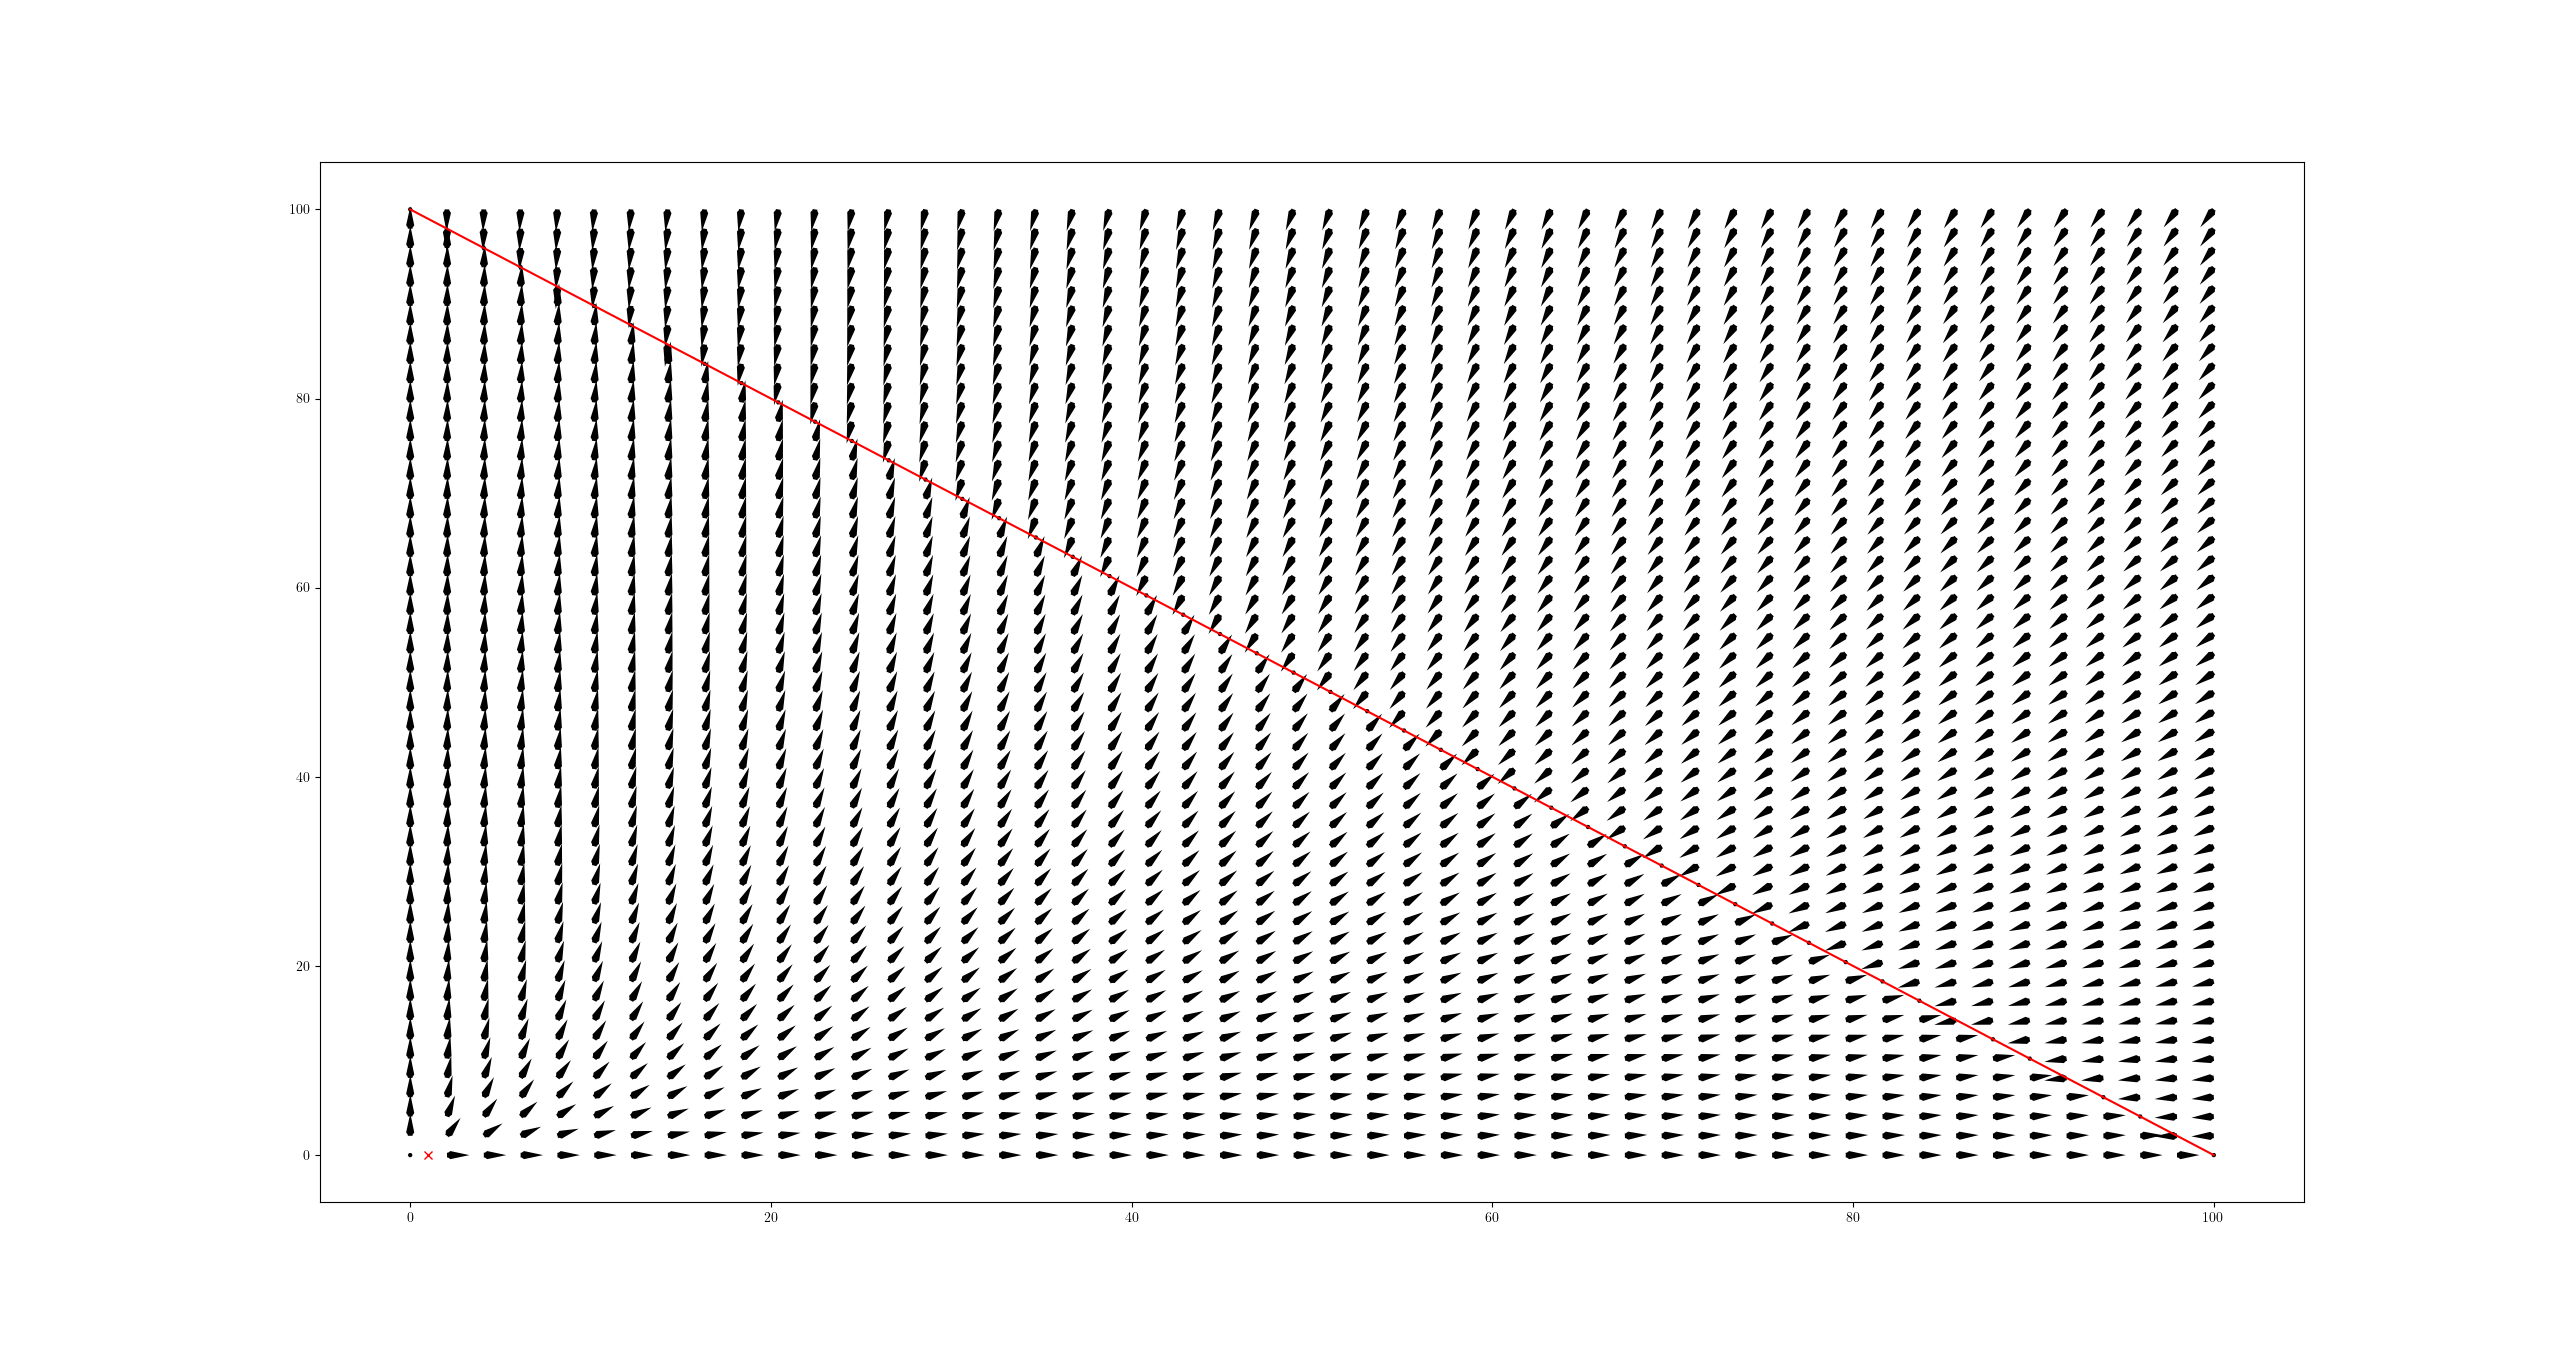
\includegraphics[width=1\linewidth]{plots/vector_field.png}
    \caption{Vector field plot for Eq \ref{eqs:adimensional_two_state_model}}
    \label{fig:vector_field_2st}
\end{figure}


The trajectory by which the system approaches this "attractor" depends on the initial conditions, as it can be seen in Figure \ref{fig:2st_vector_fiel_with_trajectory}. Figure \ref{fig:2st_vector_fiel_with_trajectory} shows indeed the trajectory in the phase space for a set of parameters with an appropriate order of magnitude inferred by comparison with the experimental data (see next section).  In the first days of the experiment,  the population growth is mostly sustained by the founder strain. Consecutive dilutions shift the initial point of the new sub-trajectories, and cause a rapid increase for the mutant population, which after around 15 days takes over the system. Nonetheless, the founder strain does not extinguish and there is a remnant population of founder strain, in agreement with the experimental data.
Furthermore, we observe that once the system reaches the attractor line, it does not fluctuate and the only way for it to reset is through the serial dilutions.

\begin{figure}[H]
    \centering
    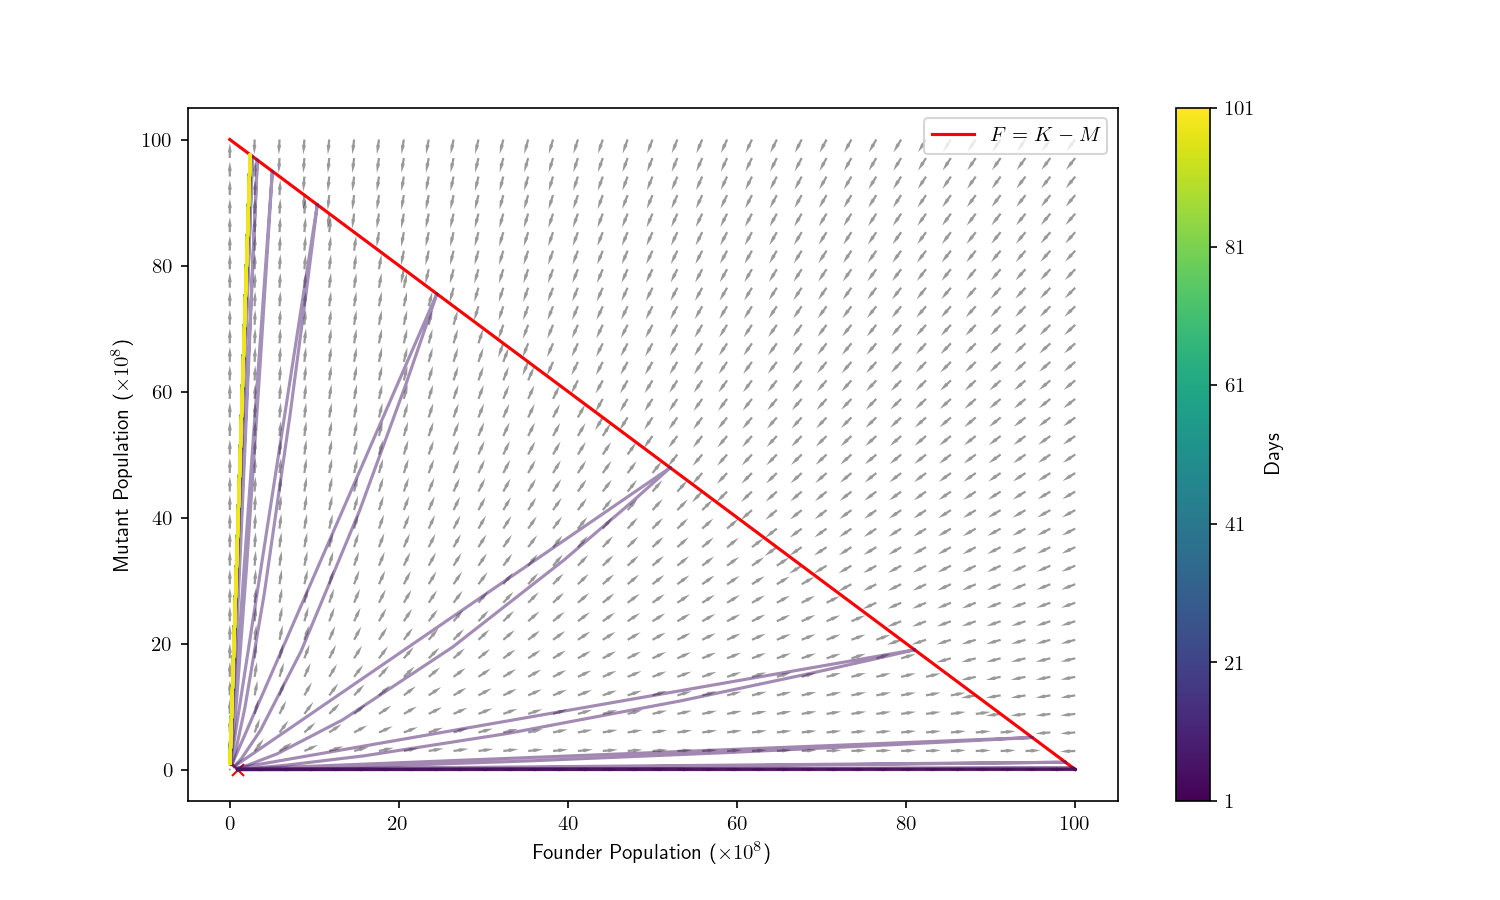
\includegraphics[width=1\linewidth]{plots/vector field with trajectory.png}
    \caption{Phase space trajectory for the two-state system. The colors indicate the day of the experiment, darker colors indicate the earlier days and brighter the latter ones. The system rapidly goes from the initial state with mostly founders to the final state where there is coexistence between mutant and founder, with a higher abundance of the former.}
    \label{fig:2st_vector_fiel_with_trajectory}
\end{figure}


\subsection*{Methods}

For computational convenience, in all the calculations we re-scaled the population by a factor of $10^8$. Hence, the reported carrying capacity of $K = 10^2$ for the simulations, corresponds to $K = 10^{10}$ in the real experiment, and so on.

All the computational work was done in Python 3.11.7 and Mathematica 3.11.7. 
Below we include a list of the relevant Python packages required to reproduce the results in this work
\begin{itemize}
\item \verb|numpy| v1.26.4
\item \verb|matplotlib| v3.8.2
\item \verb|numbalsoda| v0.3.5
\item \verb|scipy| 1.12.0
\end{itemize}

Numerical solution of ODE's was done with the \verb|lsoda| integrator from \verb|numbalsoda| and \verb|lsoda_sig| to compile the equations in C and speed up code exceution


\paragraph{Bayesian inference}
For Bayesian inference, I first used the MCMC implemented in python's \verb|emcee| package. This choice was purely based on familiarity with the package and the simplicity of its implementation. I then used the ABC implementation in PyMC v5.10.4 with the \verb|sample_smc| function. I chose 8 chains running on 4 cores of the M2 chip, the distance function is set to \verb|laplace| and the tolerance is $0.001$


\paragraph{Determining convergence times}
To determine the convergence of the system to a steady state, where each bottleneck leads to the repetition of an evolution cycle identical to the previous one, we calculate the area under the population curves using the Simpson's method implementation in \verb|scipy.integrate.simpson|. In more detail, the procedure above is described by
\begin{equation}
	\vec{A}_n = \int_n \{F_n(t),M_n(t)\} \dd t,
\end{equation}

where $n$ represents a day in the experiment
\begin{equation}
	\|\vec{A}_n - \vec{A}_{n-1} \| < \epsilon
\end{equation}
where $\|\bullet\|$ is the euclidean distance. When this condition is satisfied for three consecutive days $(n, n+1, n+2)$ we say that the system has reached the steady state.


\section{Parameter estimates}


\subsection{Replication rates from OD growth curves}

% Expand here on how parameters were estimated from growth curves
% Mention multiple scattering regime and include reference
%\section{Evolution experiment plot}



Values for the replication rates can be inferred using data from independent OD growth curves. Figure \ref{fig:gc_wt} shows the typical shape of these curves. A distinct feature of these plots is the near linearly-increasing portion that happens after the initial exponential growth, as opposed to the expected plateau due to finite resources. Contrary to what we had previously hypothesized, this linear increase is likely not due to evaporation. This behavior has in fact been previously observed \cite{stevenson_general_2016} and is instead attributed to the effects of multi-scattering arising in samples with high bacterial concentration. While this effect is controlled by subsequent dilutions when measuring the OD of a single sample using a spectrophotometer, the same precaution cannot be taken when using a 96 well plate-reader. To make sure that we stayed in the single scattering regime, where the number of bacteria is proportional to OD values, we chose to work with measurements below an OD threshold of 0.4.

\begin{figure}[H]
    \centering
    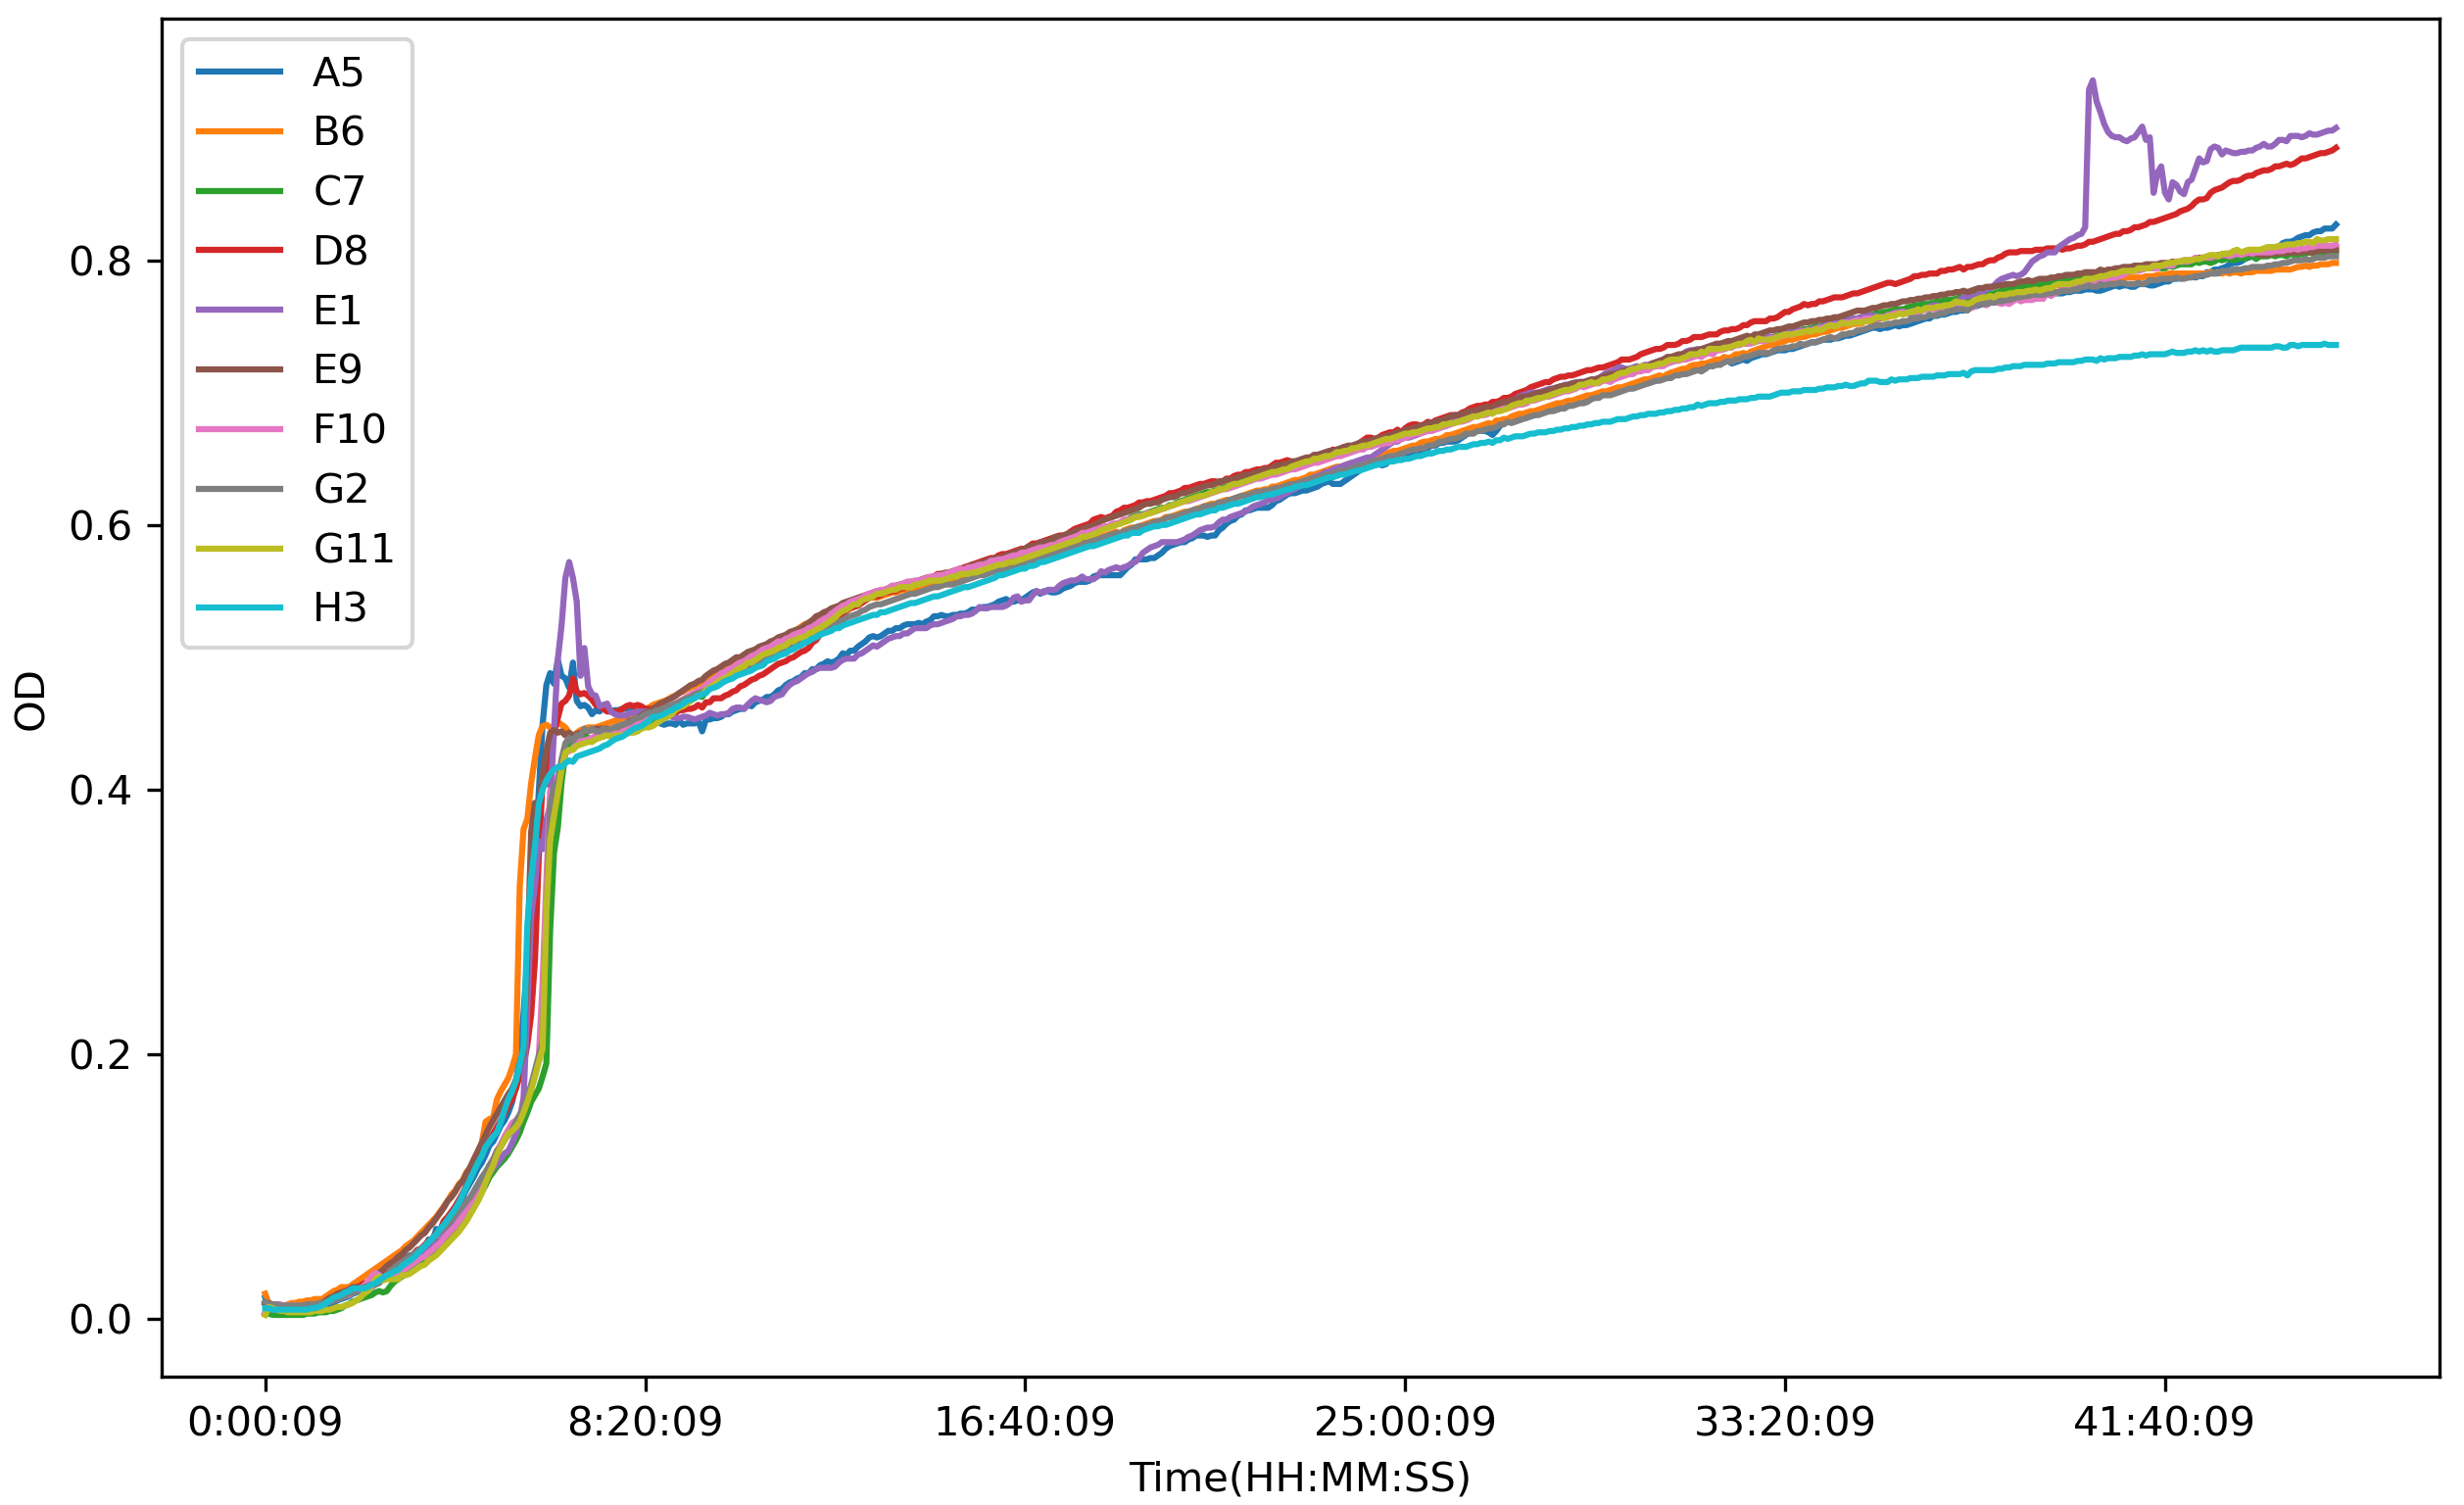
\includegraphics[scale = 0.7]{plots/gc.png}
    \caption{Growth curves for the wild type strain. Each curve represents a position in the 96 well plate}
    \label{fig:gc_wt}
\end{figure}

Determining growth rates from OD data is a process trickier than it looks; some of the subtleties are discussed in \cite{ghenu_challenges_2024,krishnamurthi_new_2021}. 
Based on this literature,  we chose to fit a generalized logistic function, 
\begin{equation}
    OD(t) = \frac{A}{\left(C + Q\exp{-Bx}\right)^\frac{1}{\nu}},
    \label{eq:generalized_logistic}
\end{equation}
to OD data for each plate's position, using all the data in the OD range $[0-0.4]$. The fit was done with Scipy's optimize function, and further verified with lmfit package in python. 

It is possible to make a parallel with the parameters in \ref{eq:generalized_logistic} and the Logistic and Richardson models as proposed in \cite{ghenu_challenges_2024}. Table \ref{tab:parameters_correspondence} shows the dependence between parameters of the different models:

\begin{table}[H]
    \centering
    \begin{tabular}{|c|c|}
    \hline
    Logistic     & Richards\\
    \hline
    $\mu = B$     & $\mu = -\frac{B}{\nu}$\\
    $K = \frac{K}{K-1}Q$     & $K = A$\\
    $N_0 = \frac{1}{k-1}Q$     & $N_0 = \left(Q+1\right)^\frac{-1}{B}$\\
    $\nu = 1$     & $\nu = -B$\\
    $C = 1$ & $C = 1$\\
    \hline
    \end{tabular}
    \caption{Correspondence between the parameters for the Logistic and Richards models in \cite{ghenu_challenges_2024} and the generalized logistic model (Eq \ref{eq:generalized_logistic}) used to fit OD curves}
    \label{tab:parameters_correspondence}
\end{table}


It is important to point out that this parallel holds only under the assumption that in the single scattering regime, OD values are proportional to the number of cells, $N$. In general, the relation between OD values and the number of cells is not well studied, it often requires calibration from the equipment used for each bacterial strain \cite{mira_estimating_2022}. Alternative experimental methods for estimating bacterial population from OD values have been suggested \cite{beal_robust_2020}; however, for the purpose of this project, we are not concerned with this problem directly. It is enough to restrict ourselves to the the single scattering regime, where we assume a linear relation between OD and N.


\subsection{Other parameters from morphological data fitting}

The evolution experiment is carried out with the following conditions: 
\begin{itemize}
    \item The carrying capacity is set to the maximal bacterial density measured at the end of one evolution cycle, $K = 10^{10} \text{cells}$ \textbf{(TO CHECK!!)}
    \item The estimated initial cell density is $N_0= 10^9 \ \text{cells/mL}$ in 100 $\mu \text{L}$ of solution
    \item After each day, 1\% of the solution is used to start the next culture
    \item The founder strain is the named \textit{delserCGA} and the reference mutant we used for estimating the mutant replication rate is \textit{M2lop}
\end{itemize}

\subsubsection{Getting good orders of magnitude with visual fitting}

After having estimated the replication rates with the independent OD growth curves, we still need good estimates for the values of the transition rates $(\Tilde{\mu}_{FM}, \Tilde{\mu}_{MF})$ to use as priors for the Bayesian inference using morphological data (see next subsection).
To gain some understanding on the behavior of the solutions to Eq. \ref{eqs:adimensional_two_state_model} with respect to the parameters, I initially solved the two state system for different values of $(\Tilde{\mu}_{FM}, \Tilde{\mu}_{MF})$,  fixing the value of $\alpha$ with the growth curve data. This naive search provided some useful observations.

I found that varying $\Tilde{\mu}_{FM}$ shifts the day at which the final populations of mutant and founder are the same (the crossing point), without noticeably changing the ratio of the two populations at the end of the experiment, meaning that this transition rate determines how fast the founder population disappears. Qualitatively, this makes sense, considering that at the beginning of the experiment, there are no mutants, therefore the transition rate from $F$ to $M$ is an important contributor to the quick appearance of a mutant population.

On the other hand, varying $\Tilde{\mu}_{MF}$ seems to strongly determine the final fraction of population at the end of the experiment. Figure \ref{fig:effect_of_varying_mu_mf} illustrates this behavior: for a small $\Tilde{\mu}_{MF}$, the proportion of founder in the final state is considerably higher than the proportion of mutants. As $\Tilde{\mu}_{MF}$ increases, the final founder proportion increases as well. This might indicate that this parameter is a key determinant for the fate of each strain, and in consequence of the proposed set of hypotheses. 

\begin{figure}
    \centering
    \begin{subfigure}[b]{0.4\textwidth}
    \centering
    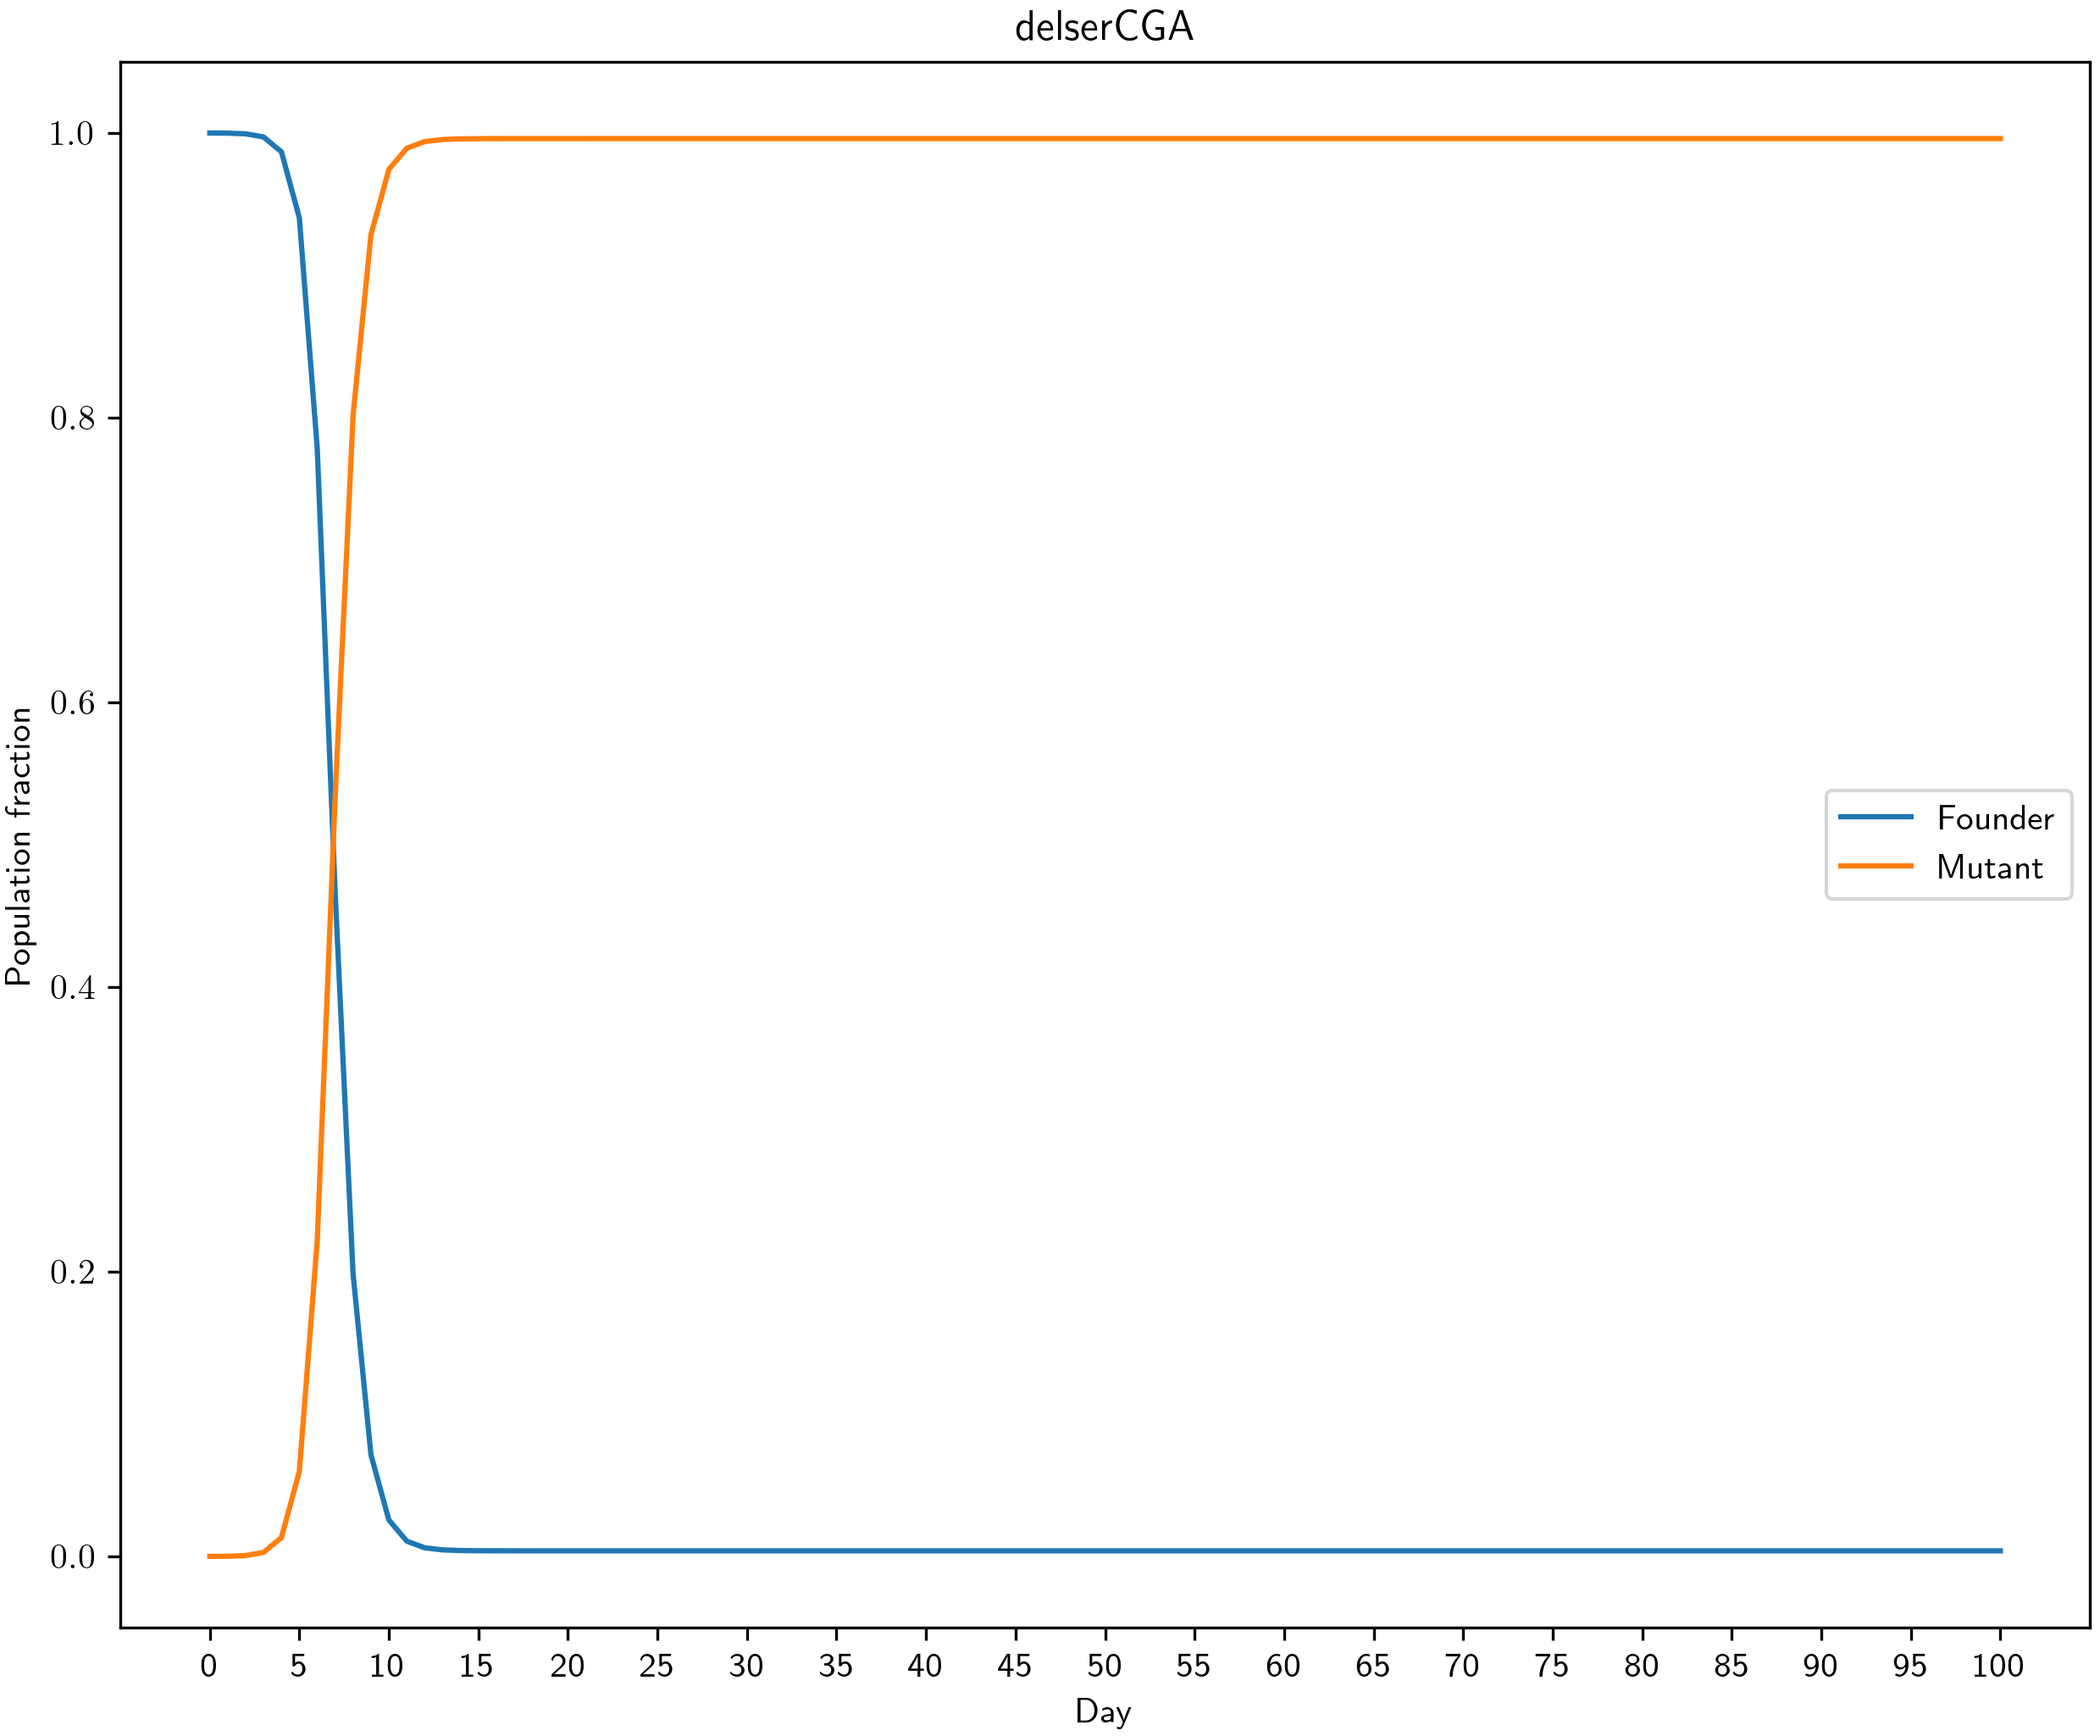
\includegraphics[scale=0.4]{plots/two_state_small_mu_mf.png}
    \end{subfigure}
    \hfill
    \begin{subfigure}[b]{0.4\textwidth}
    \centering
    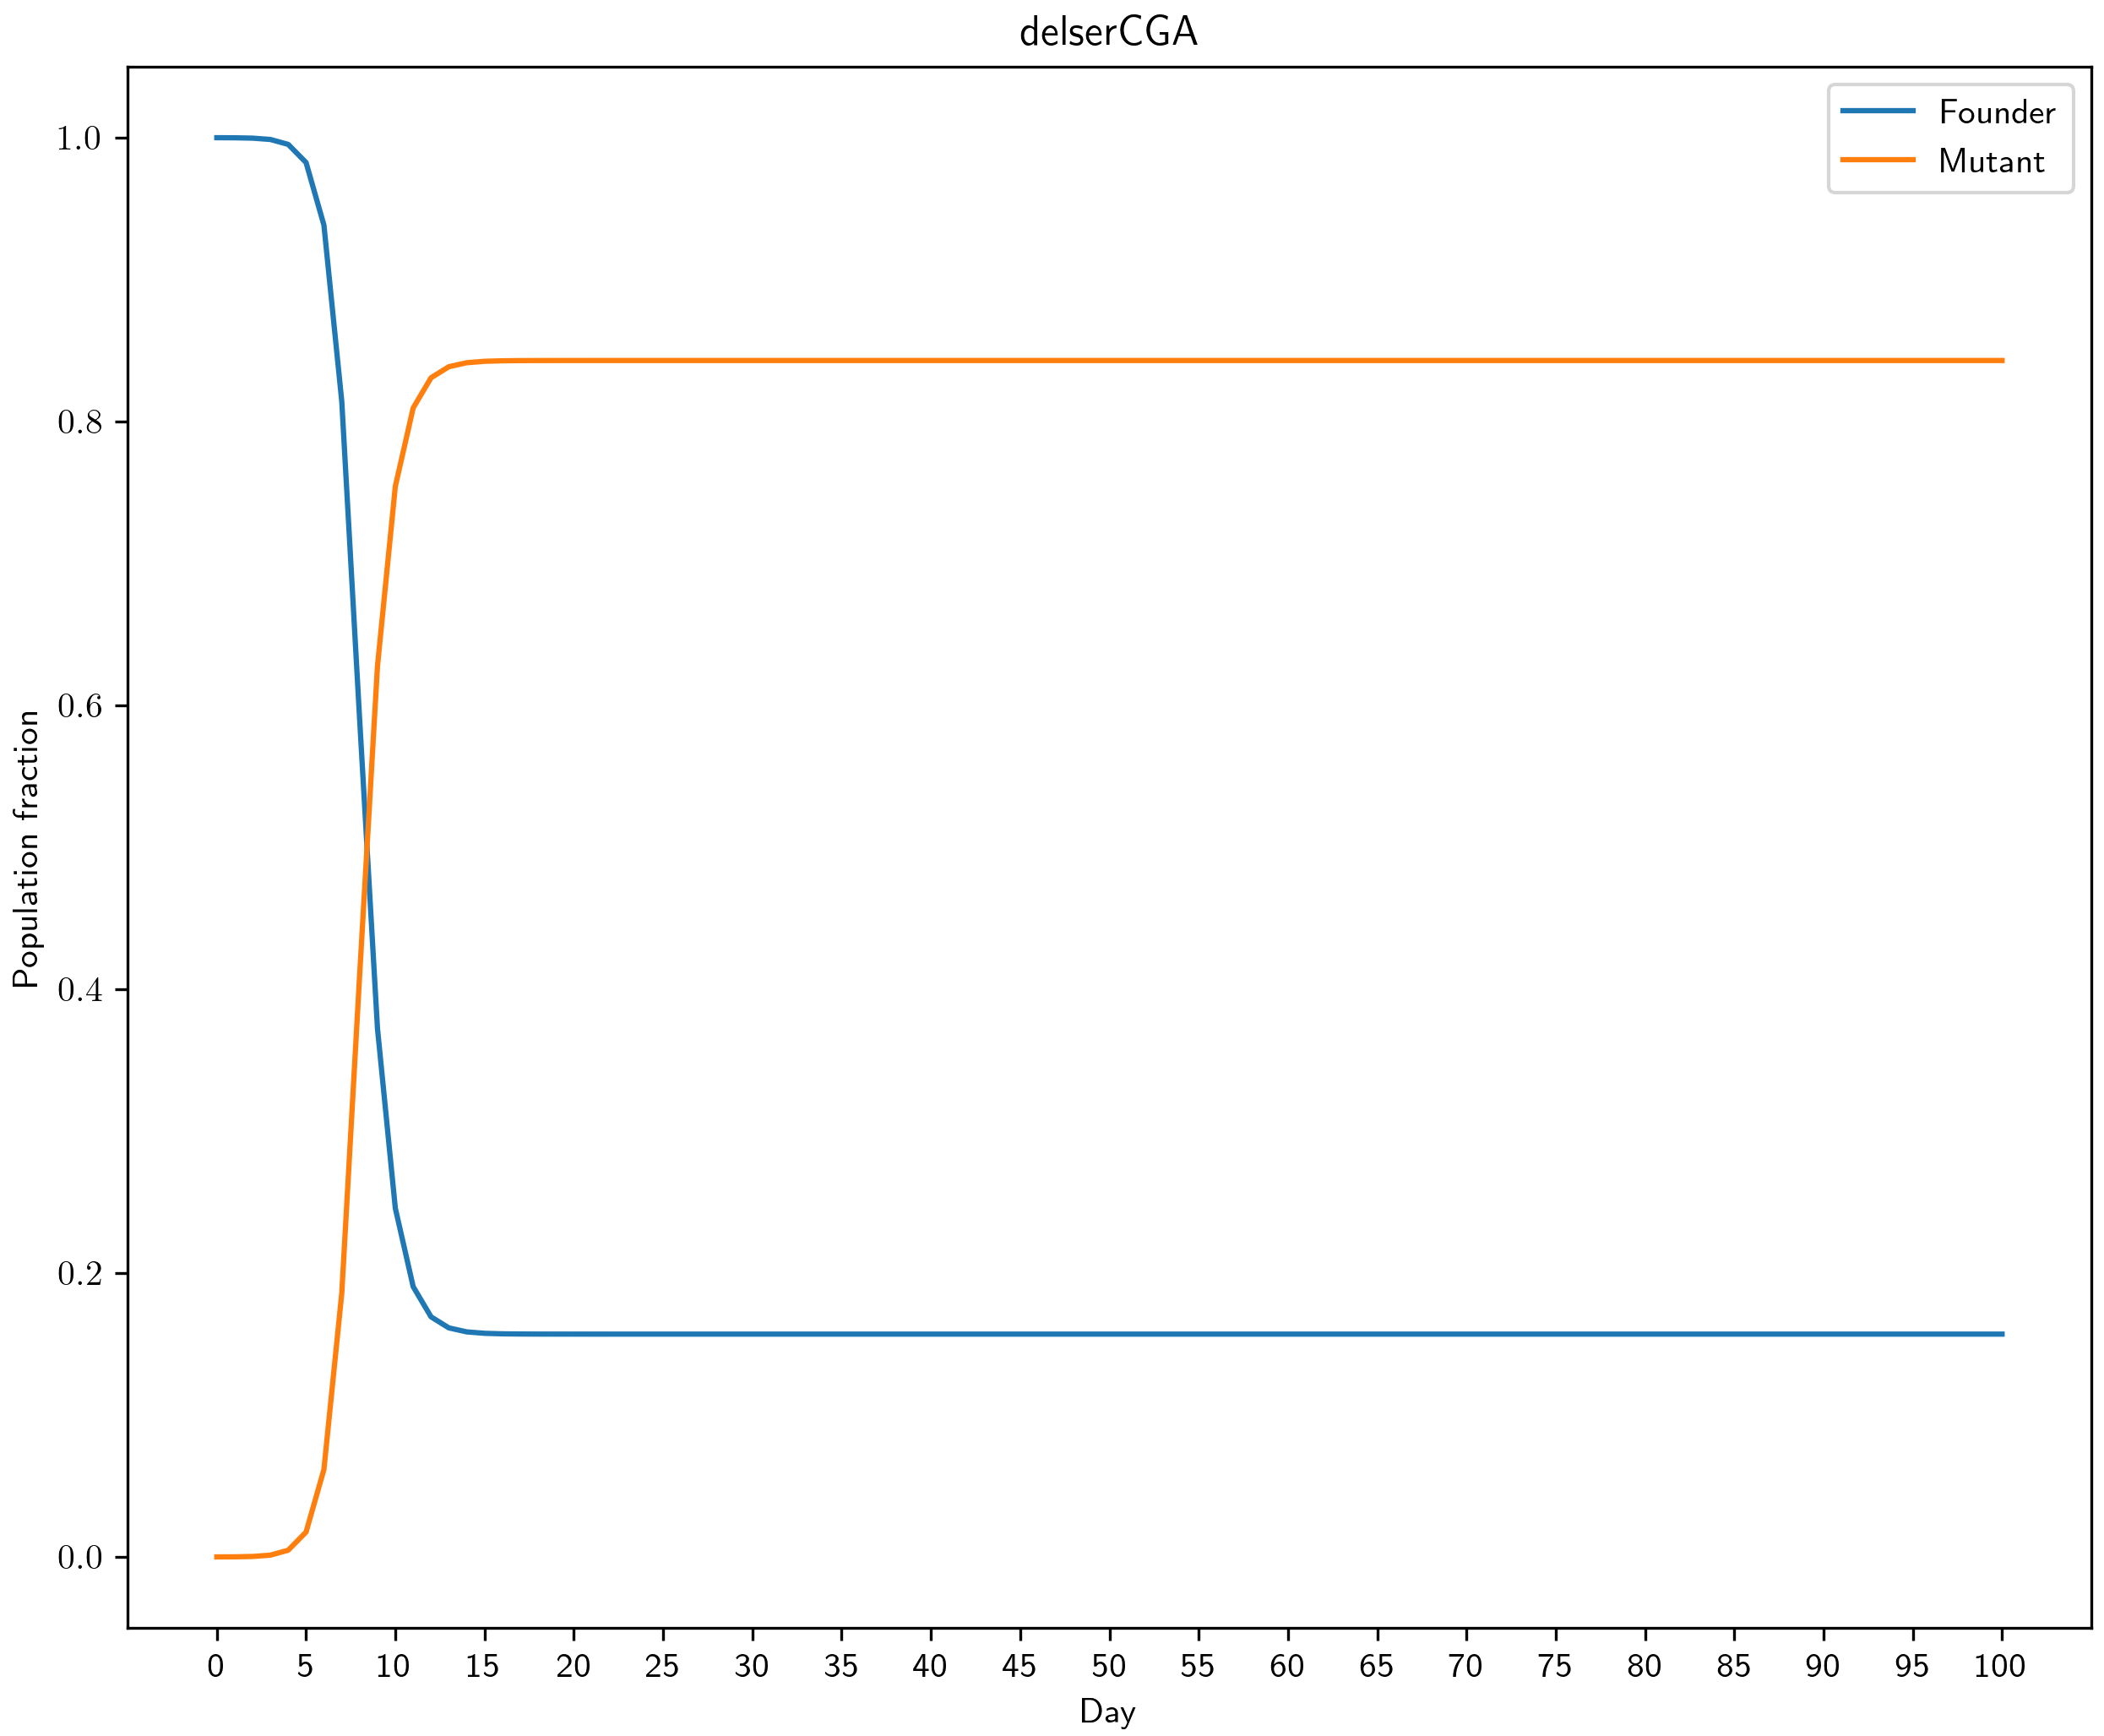
\includegraphics[scale=0.4]{plots/two_state_big_mu_mf.png}
    \end{subfigure}
    \caption{Effect of varying $\Tilde{\mu}_{MF}$ on the population fraction behavior in the evolution experiment. Both panels have fixed values for $\Tilde{\mu}_{FM}$ and $\alpha$. $\Tilde{\mu}_{MF} = 0.001 * \ln{2}$ (left) and $\Tilde{\mu}_{MF} = 0.4 * \ln{2}$ (right). }
    \label{fig:effect_of_varying_mu_mf}
\end{figure}

An important observation here is the difference in the order of magnitude for the transition rates,   $\Tilde{\mu}_{MF}$ has a stronger influence around $10^{-4}$, whereas $\Tilde{\mu}_{MF}$ does it around $10^{-9}$. Nonetheless, this behaviour is similar to the one described in \cite{reams_duplication_2010}.

Now, when $\alpha$ is allowed to vary, it exhibits a rather interesting behavior. In the limit where $\alpha \rightarrow 1$ there is no notorious shift in the population from founder to mutants; they remain close to their initial values, at least in a time frame suitable for an experiment. This behavior completely changes as $\alpha$ increases. As soon as $\alpha  \rightarrow 2$ the mutant population quickly takes over the system and remains like that for the rest of the experiment.


\begin{table}[H]
    \centering
    \begin{tabular}{|c|c|}
        \hline
        Parameter & Value\\
         \hline
         $r_f$& $4.0603\times 10^{-2} \ \text{min}^{-1}$\\
         $r_M$& $5.4478\times 10^{-2} \ \text{min}^{-1}$\\
         $\mu_{FM}$ & $4.25\times 10^{-9}\frac{\text{mutation}}{\text{generation}}$\\
         $K$ & $10^{10}$\\
         \hline
    \end{tabular}
    \caption{Initial parameters for the toy model}
    \label{tab:initial_parameters_two_state_model}
\end{table}


Now,  in Fig \ref{fig:population_frac_2st} I look at the solution for the two state system\footnote{Even though we illustrate the behavior with replicate 1, the discussion is still valid for the other replicates as their values almost the same}, using the parameter values that are indicated in table \ref{tab:initial_parameters_two_state_model} -- selected by tuning the parameters manually. %Is that correct? Ask Miguel? Yes
The sharp drops in the proportions of founder and mutant are captured, as well as the remnant founder population in the equilibrium state.

\begin{figure}[H]
    \centering
    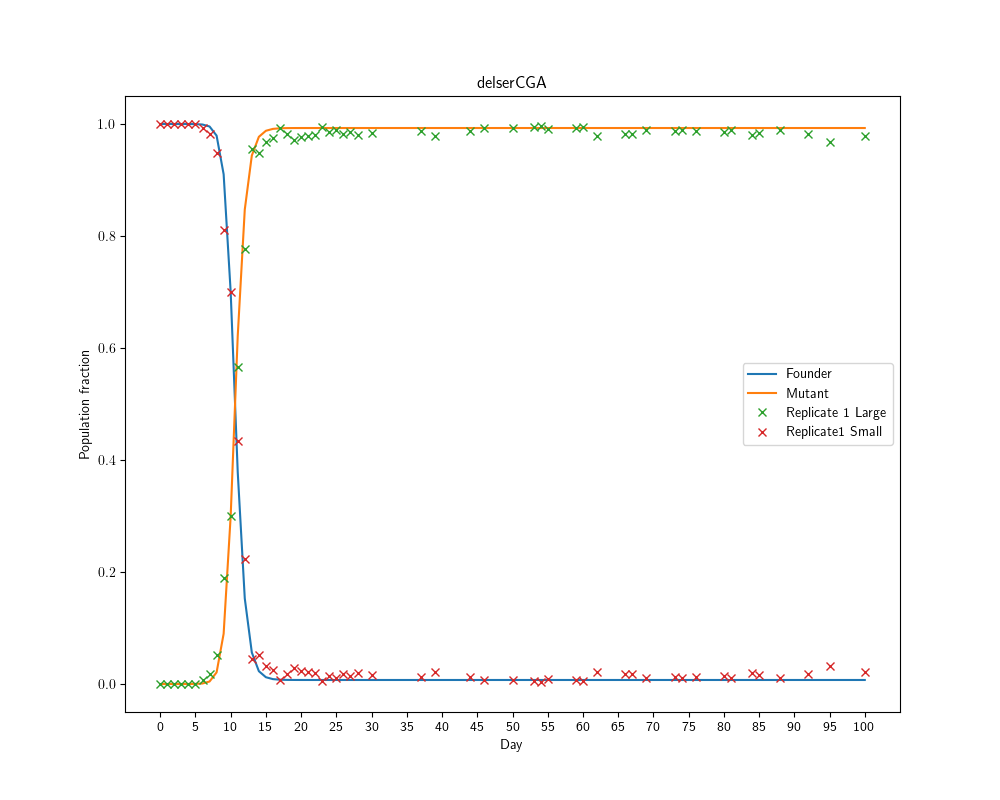
\includegraphics[width=1\linewidth]{guessed_params_2st_evolution_plot.png}
    \caption{Proportions of founders and mutants for the two-state system. The parameters used were $K = 10^2$, %%%WHAAAAT? Ask Miguel --> because everything is rescaled by 10^8
$\alpha = 1.34187, \Tilde{\mu}_{FM} = 0.0039\times 10^{-6}, \Tilde{\mu}_{MF} = 1.26611\times 10^{-3}$. The solid lines are the theoretical predictions for the populations through the duration of the experiment. The x indicate the measured values of the populations proportions for small and large colonies in Replicate 1. Large colonies are interpreted as encompassing all types of mutations, while small colonies are understood as founder colonies.}
    \label{fig:population_frac_2st}
\end{figure}

\subsubsection{Bayesian Inference for the two state model}

My initial approach to simplify the number of parameters to determine was to assume that the replication rate of the mutant was known, for this I used the value of the reported rate for \textit{M2lop} $(r_M = 0.05448 \text{ replication/min})$. By playing with the parameters I had some intuition about a range where the solution fit the experimental results (see fig. \ref{fig:population_frac_2st}). I first chose to use Affine Invariant MCMC to determine the transition rates. With a uniform prior between 0 and 1 , the posterior distribution fails to reproduce similar experimental measurements.

Given that the initial flavor of MCMC was not successful at fitting the parameters to the experimental data, I switched to an Approximate Bayesian Calculation (ABC). This new approach yielded satisfactory results shown in Figure \ref{fig:abc_2st_posterior}. This parameter distribution supports the values encountered previously for $\alpha$, and the difference between the orders of magnitude of mutation and loss rates is close to the behavior described in \cite{reams_duplication_2010}. 
 
\begin{figure}[H]
	\centering
    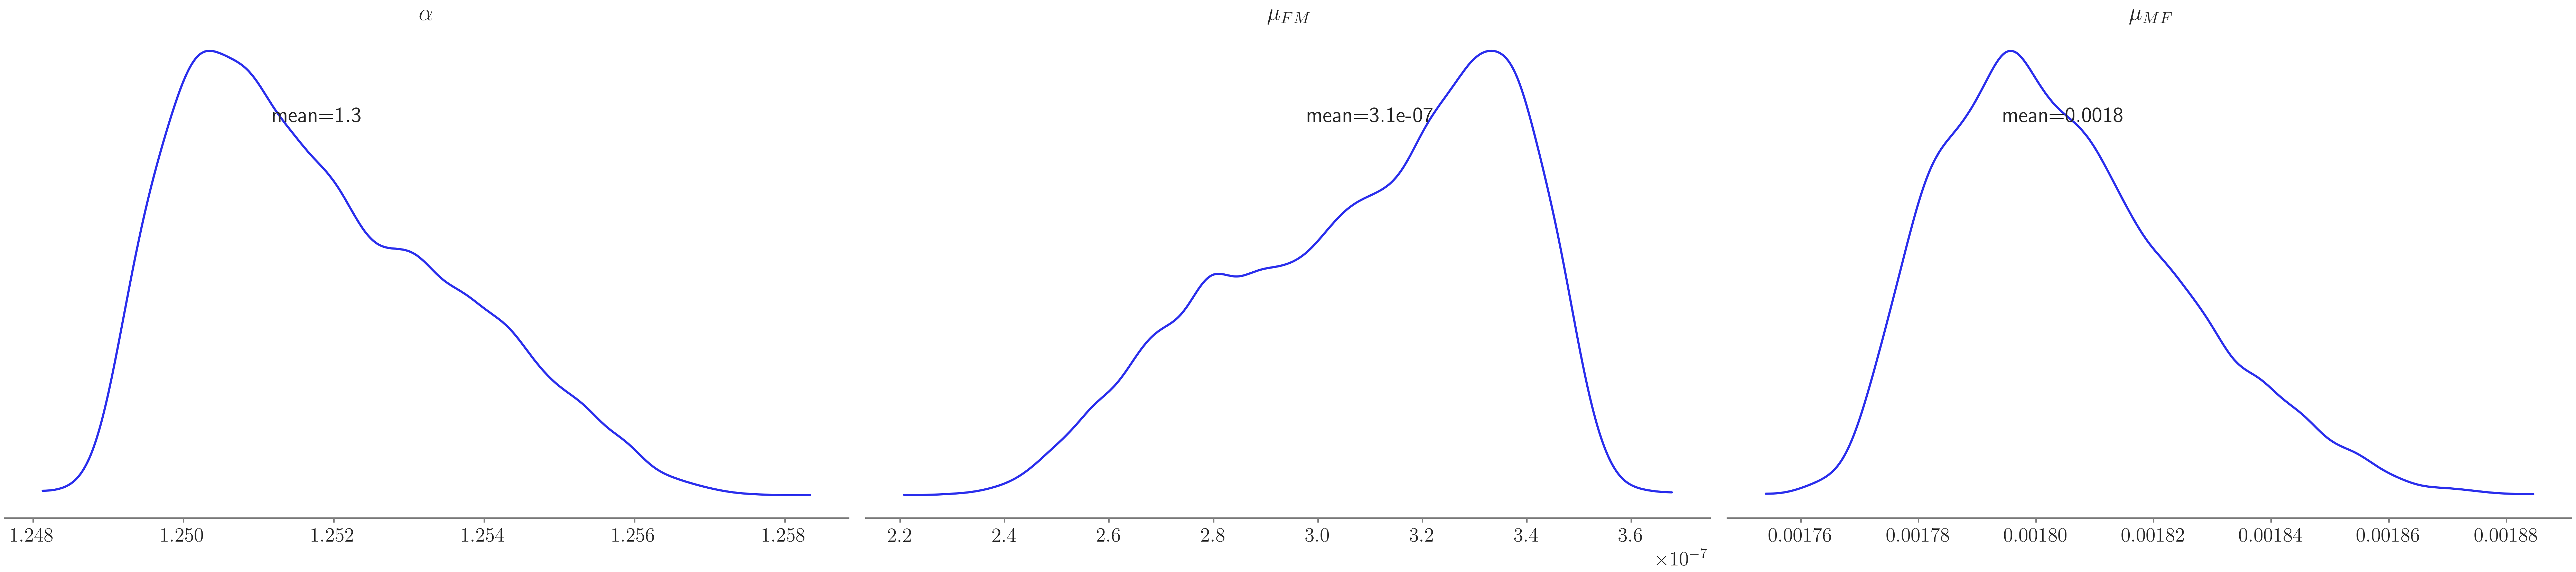
\includegraphics[scale=0.3]{plots/abc_2st_posterior.png}
    \caption{Posterior distribution for the parameters of the two state model inferred with ABC}
    \label{fig:abc_2st_posterior}
\end{figure}
Figure \ref{fig:2st_abc_fit} shows the experimental points along with the theoretical predictions (solid line) obtained by solving the model with the mean of the parameters distribution in Figure \ref{fig:abc_2st_posterior}. %ASK MIGUEL: why the mean rather than the max? --> check what people usually do
As we can see, the predictions reproduce the measured behavior of the populations, capturing the fast increase in mutants and the remnant founder population after 100 days.

\begin{figure}[H]
	\centering
    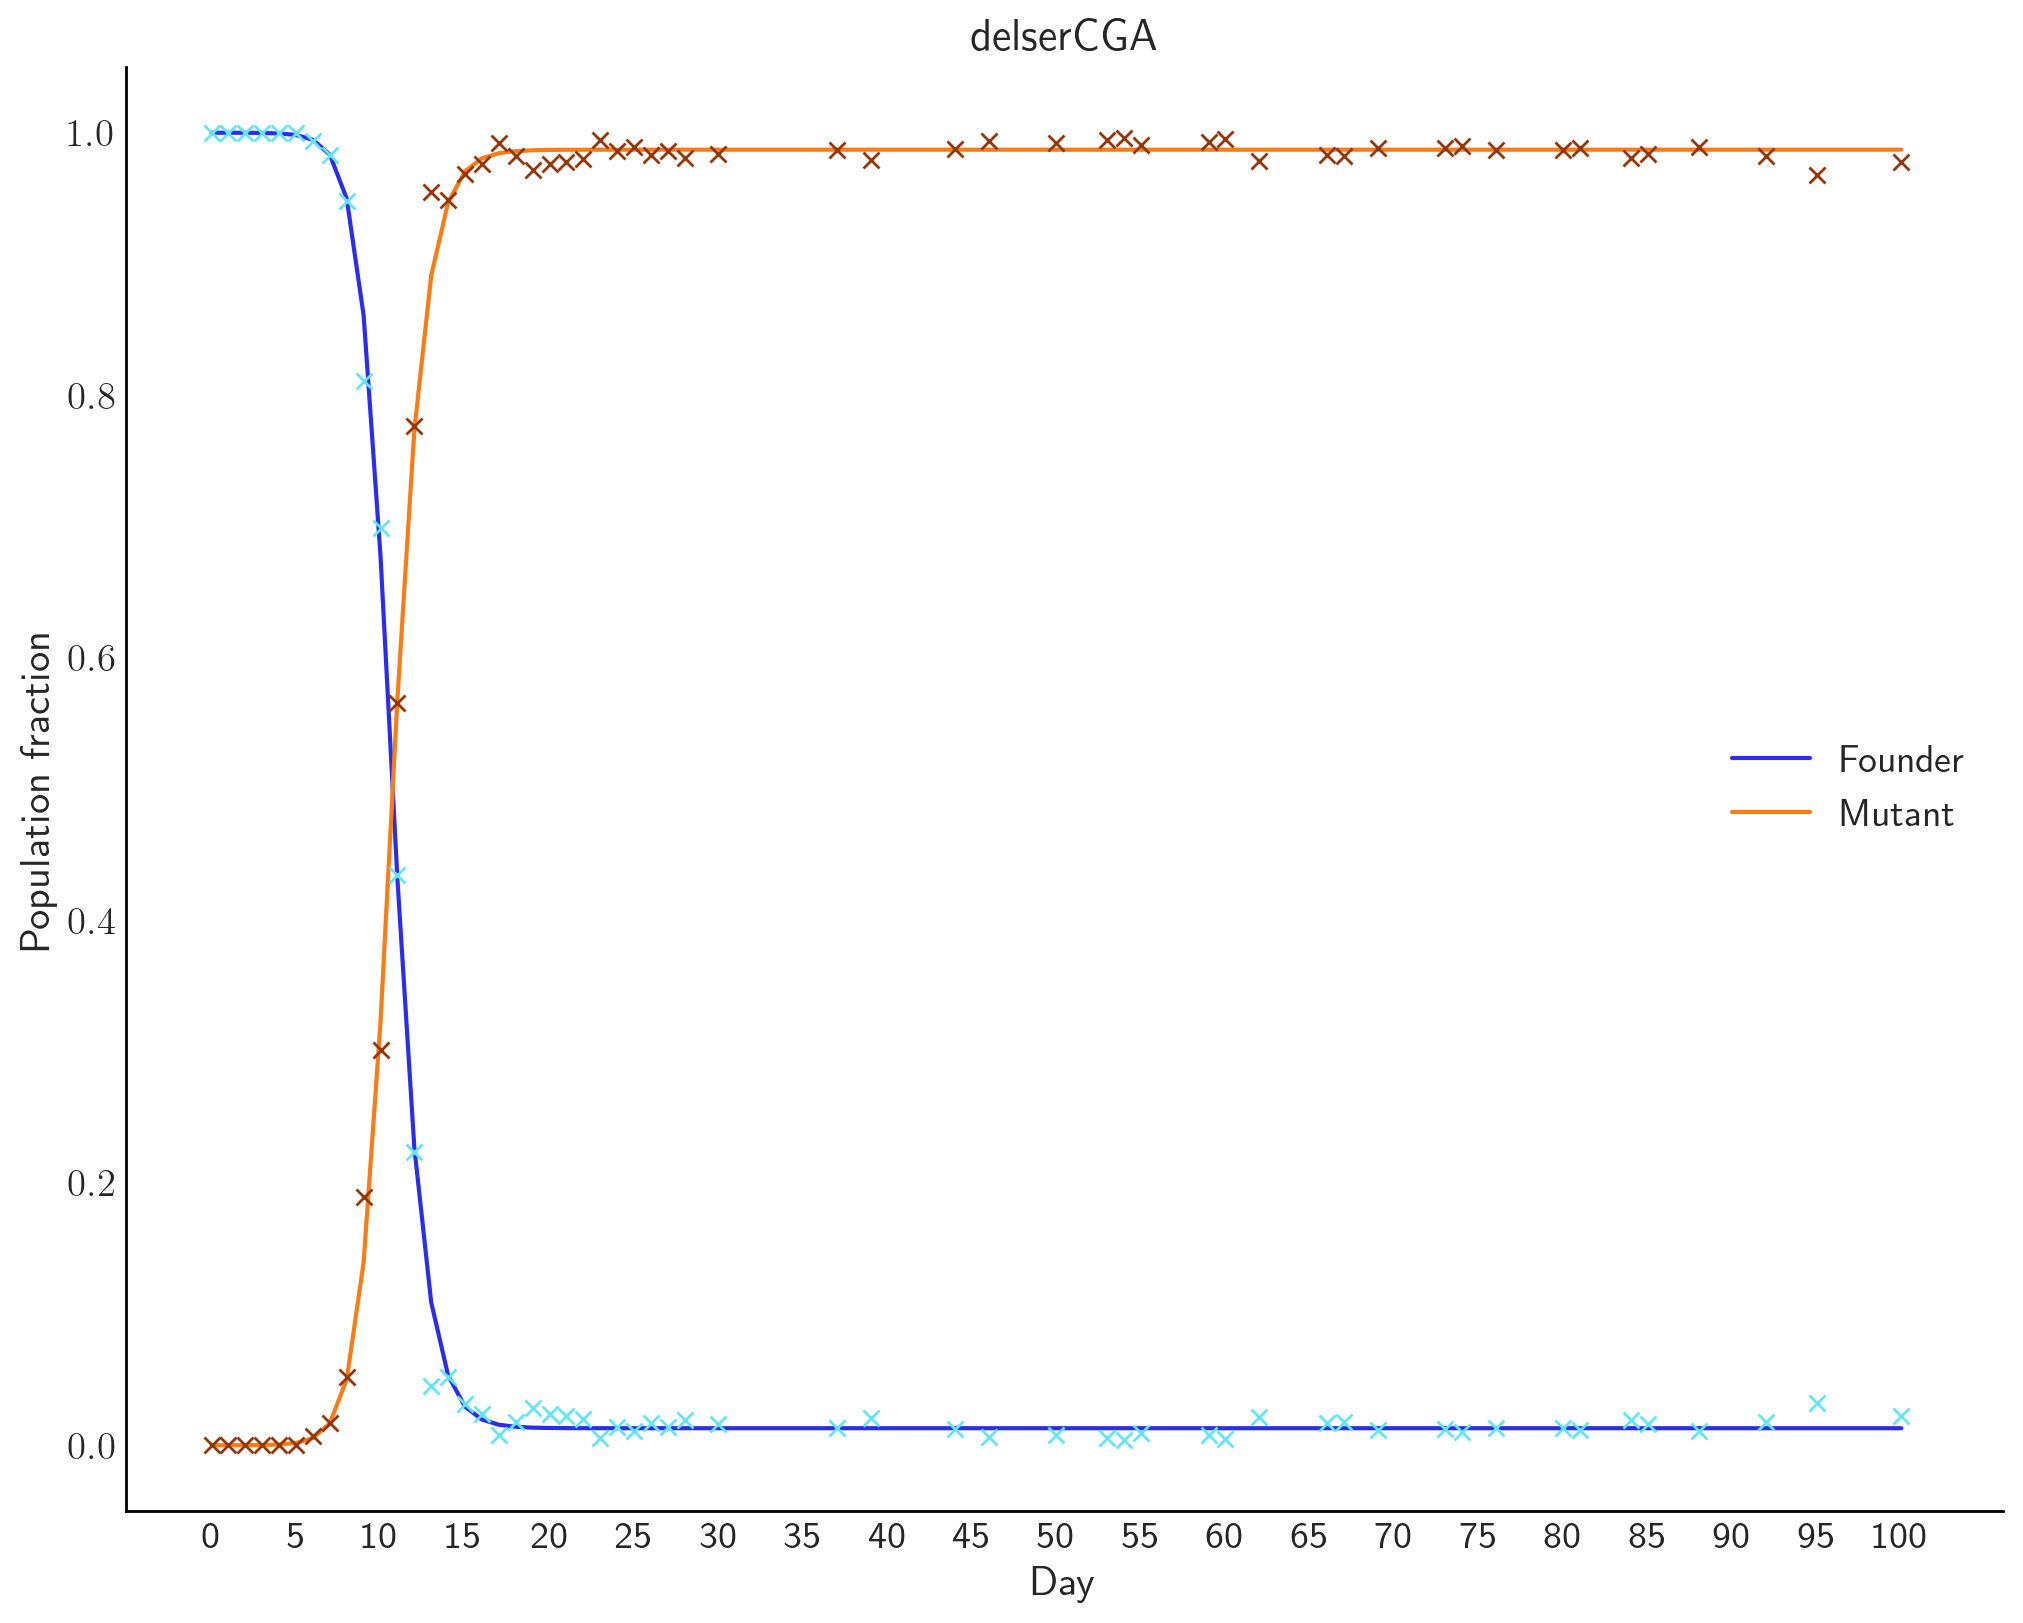
\includegraphics[scale=0.4]{plots/2st_abc_fit.png}
    \caption{The solid lines represent the theoretical evolution of the population fraction using the two state model. The x are the experimental measurements of the proportions of small and large colonies.}%Tell Miguel: ratio and proportion is not the same!
    \label{fig:2st_abc_fit}
\end{figure}

%Tell Miguel: What I miss here, is
%- the exact values for the parameters that are inferred
%- a comment on them: how does it compare with: the "manual" estimates of the previous section? with values from the literature? (the value we previously used for SNPs?) --> the orders of magnitude match


\subsubsection{Bayesian Inference for the three state model}
Let's start by writing the adimensional expression of equations \ref{eqs:three_state_model}, where time has been scaled by a factor of $r_F$

\begin{subequations}\label{eqs:adimensional_three_state_model}
\begin{align}
\dv{F}{\tau} &= \left( \left(1 - \Tilde{\mu}_{FD} - \Tilde{\mu}_{FS}\right)F + \alpha \Tilde{\mu}_{DF} D + \beta \Tilde{\mu}_{SF} S \right)\left(1-\frac{F + D + S}{K}\right)\\
\dv{D}{\tau} &=\left(  \Tilde{\mu}_{FD}F + \alpha\left(1 -\Tilde{\mu}_{DF}\right)D \right) \left(1-\frac{F + D + S}{K}\right) \\
\dv{S}{\tau} &= \left( \Tilde{\mu}_{FS}F + \beta\left(1 - \Tilde{\mu}_{SF}\right)S \right) \left(1-\frac{F + D + S}{K}\right) 
\end{align}
\end{subequations}
with $\tau = r_F t$, $\alpha = \frac{r_D}{r_F}, \beta = \frac{r_S}{r_F}$, $\Tilde{\mu}_{FD} = \frac{\mu_{F\rightarrow D}}{\ln{2}}, \Tilde{\mu}_{FS} = \frac{\mu_{F\rightarrow S}}{\ln{2}}, \Tilde{\mu}_{DF} = \frac{\mu_{D\rightarrow F}}{\ln{2}}, \Tilde{\mu}_{SF} = \frac{\mu_{S\rightarrow F}}{\ln{2}}$.
This model involves more unknown parameters than Eq \ref{eqs:adimensional_two_state_model}, thus MCMC computation time will be significantly larger as it scales with the dimensionality of the parameter space. Running an Approximate Bayesian Computation algorithm is a more suitable option, given that it doesn't involve calculating a likelihood function and the implementation chosen is well optimized. From solving Eqs \ref{eqs:adimensional_three_state_model} for different combinations of parameters and previous work with the two state model, I already had prior knowledge of at least some orders of magnitude for the parameters. In this way I define the prior probability as
\begin{subequations}
    \begin{align*}
        \alpha, \beta &\sim \mathcal{U}_{[1,2]}\\
        \Tilde{\mu}_{FD} &\sim \mathcal{N}(0,10^{-5}), \quad \Tilde{\mu}_{FD}>0 \\
        \Tilde{\mu}_{FS} &\sim \mathcal{N}(0,10^{-5}), \quad \Tilde{\mu}_{FS}>0 \\
        \Tilde{\mu}_{DF} &\sim \mathcal{N}(0,10^{-5}), \quad \Tilde{\mu}_{DF}>0 \\
        \Tilde{\mu}_{SF} &\sim \mathcal{N}(0,10^{-5}), \quad \Tilde{\mu}_{SF}>0 
    \end{align*}
\end{subequations}

The ABC calculations yield to the posterior distributions for the parameters shown in fig \ref{fig:posterior_abc_3st}.

\begin{figure}[H]
    \centering
    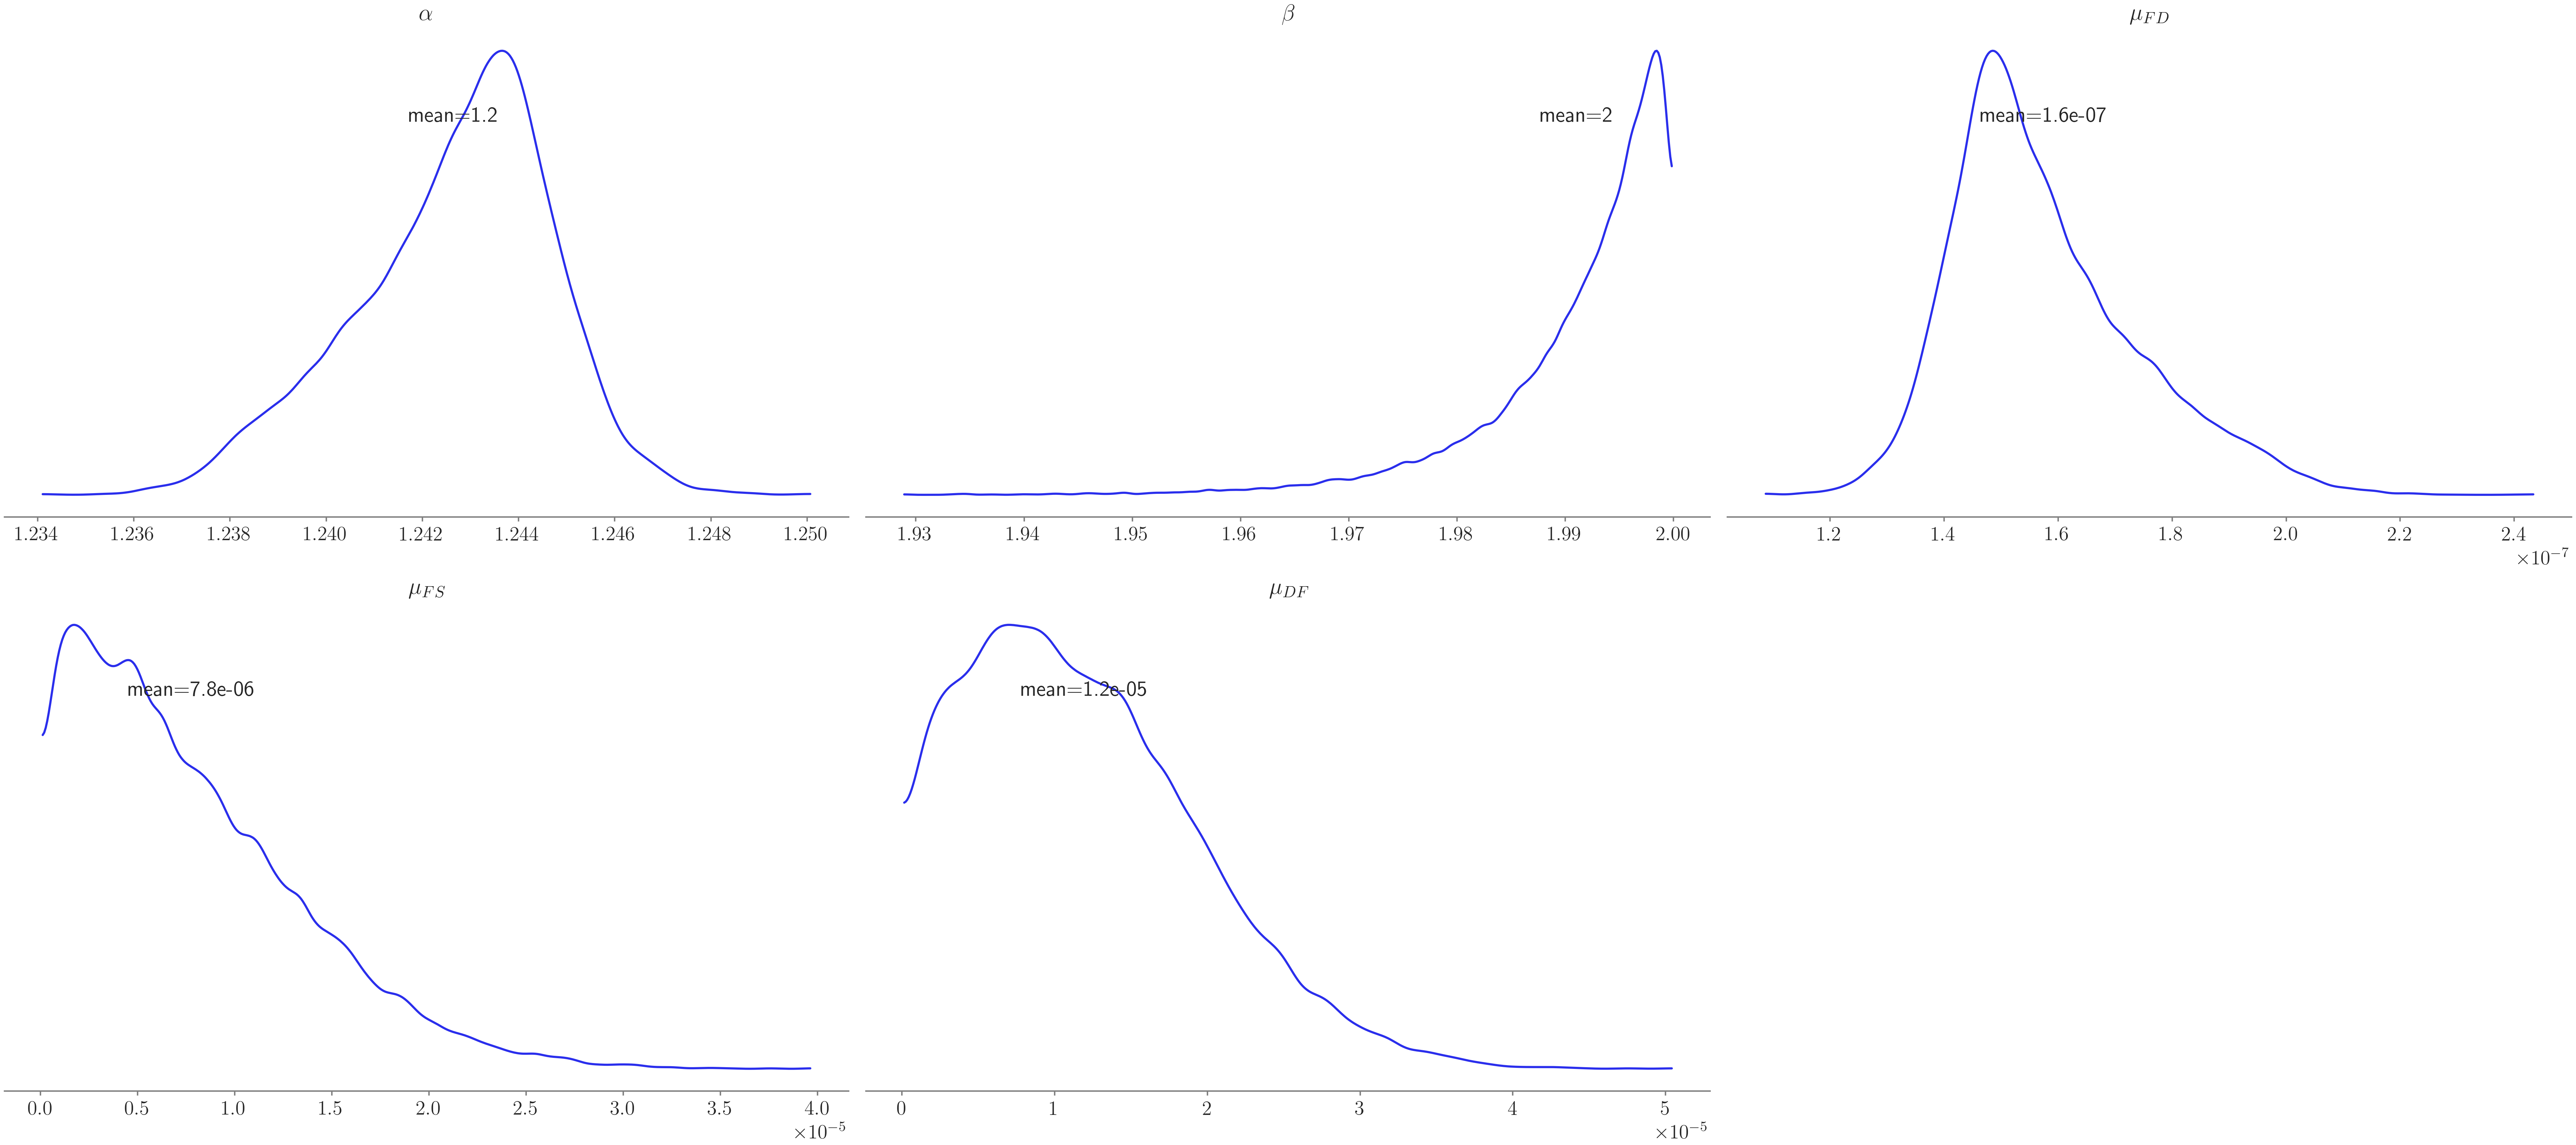
\includegraphics[width=1\linewidth]{abc_3st_posterior.png}
    \caption{Posterior distribution for parameters in Eq \ref{eqs:adimensional_three_state_model}}
    \label{fig:posterior_abc_3st}
\end{figure}

As an additional information on how well the parameter space was explored using the ABC method, the figure \ref{fig:abc_3st_param_chains} below shows the distribution of the chains followed for each parameter.

\begin{figure}[H]
    \centering
    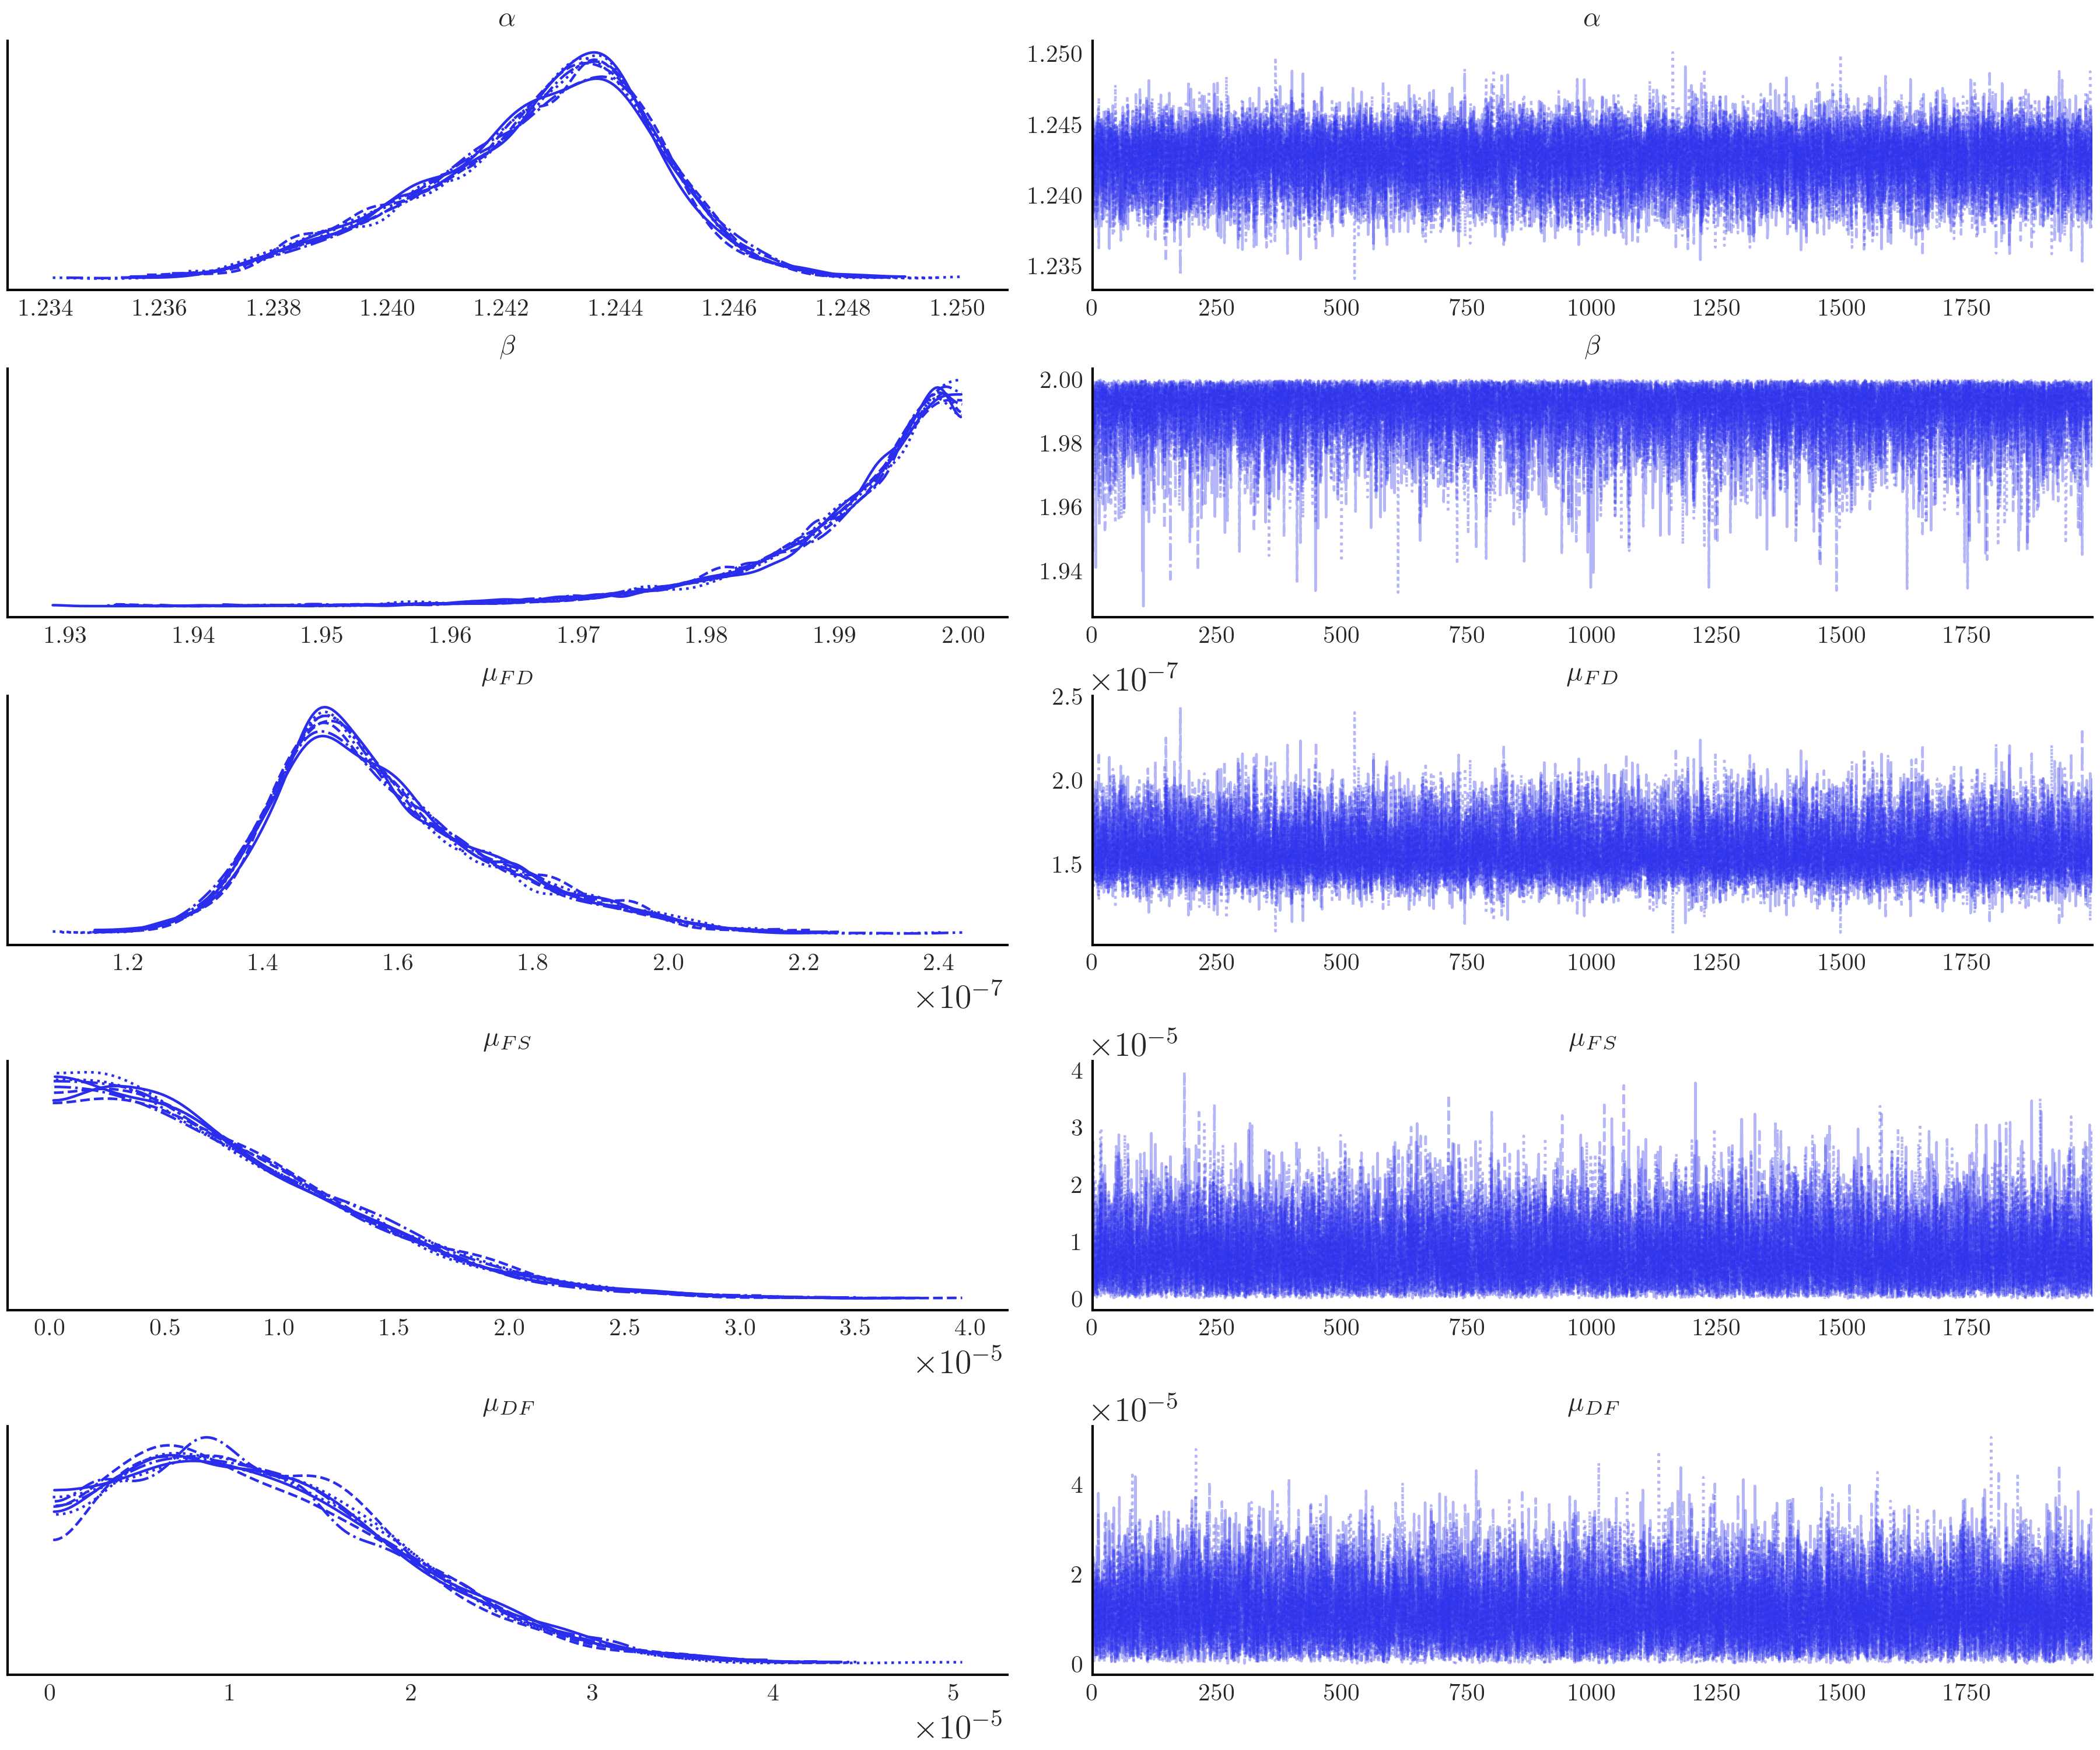
\includegraphics[width=1\linewidth]{plots/abc_3st_param_dist.png}
    \caption{Distribution of the chains for ABC results in Fig \ref{fig:posterior_abc_3st}}
    \label{fig:abc_3st_param_chains}
\end{figure}

Even though we had a value for the replication rate of the \textit{M2lop} mutant, we set it to vary in the model. Table \ref{tab:abc_3st_params} summarizes the mean and std of each obtained posterior distribution.

\begin{table}[H]
    \centering
    \begin{tabular}{c|c|c}
    \hline
    & \textbf{mean} & \textbf{std} \\\hline
     $\alpha$ & 1.2427   & $2.0 \times 10^{-3}$ \\
     $\beta$  & $1.9911$ & $8.5 \times 10^{-3}$\\
     $\mu_{FD}$    & $1.576\times 10^{-7}$ & $1.634\times 10^{-8}$ \\
     $\mu_{FS}$    & $7.811\times 10^{-6}$ & $5.804\times 10^{-6}$ \\
     $\mu_{DF}$    & $1.199\times 10^{-5}$ & $7.598\times 10^{-6}$ \\\hline
    \end{tabular}
    \caption{Statistics summary of the parameter distribution for Eq \ref{eqs:adimensional_three_state_model} from ABC results}
    \label{tab:abc_3st_params}
\end{table}

%Question to Miguel: Did you consider muSF to be 0? If yes, needs to be written explicitely. If no, why is it missing?

I choose the mean of each parameter as a representative sample of the algorithm results, and used them to numerically solve the equations. To compare with the experimental data, I sum the population fractions from Duplication and SNP strains -- this should correspond to the fraction of observed large colonies. Visually inspecting the population fractions in Fig \ref{fig:abc_3st_experiment_comparison} we can see that the prediction with the inferred parameters is close to the experimental data. Furthermore, the parameters seem to reproduce the long-time behavior of the experiment as the founder population is not completely extinct, instead there is a small remnant of it.
\begin{figure}[H]
    \centering
    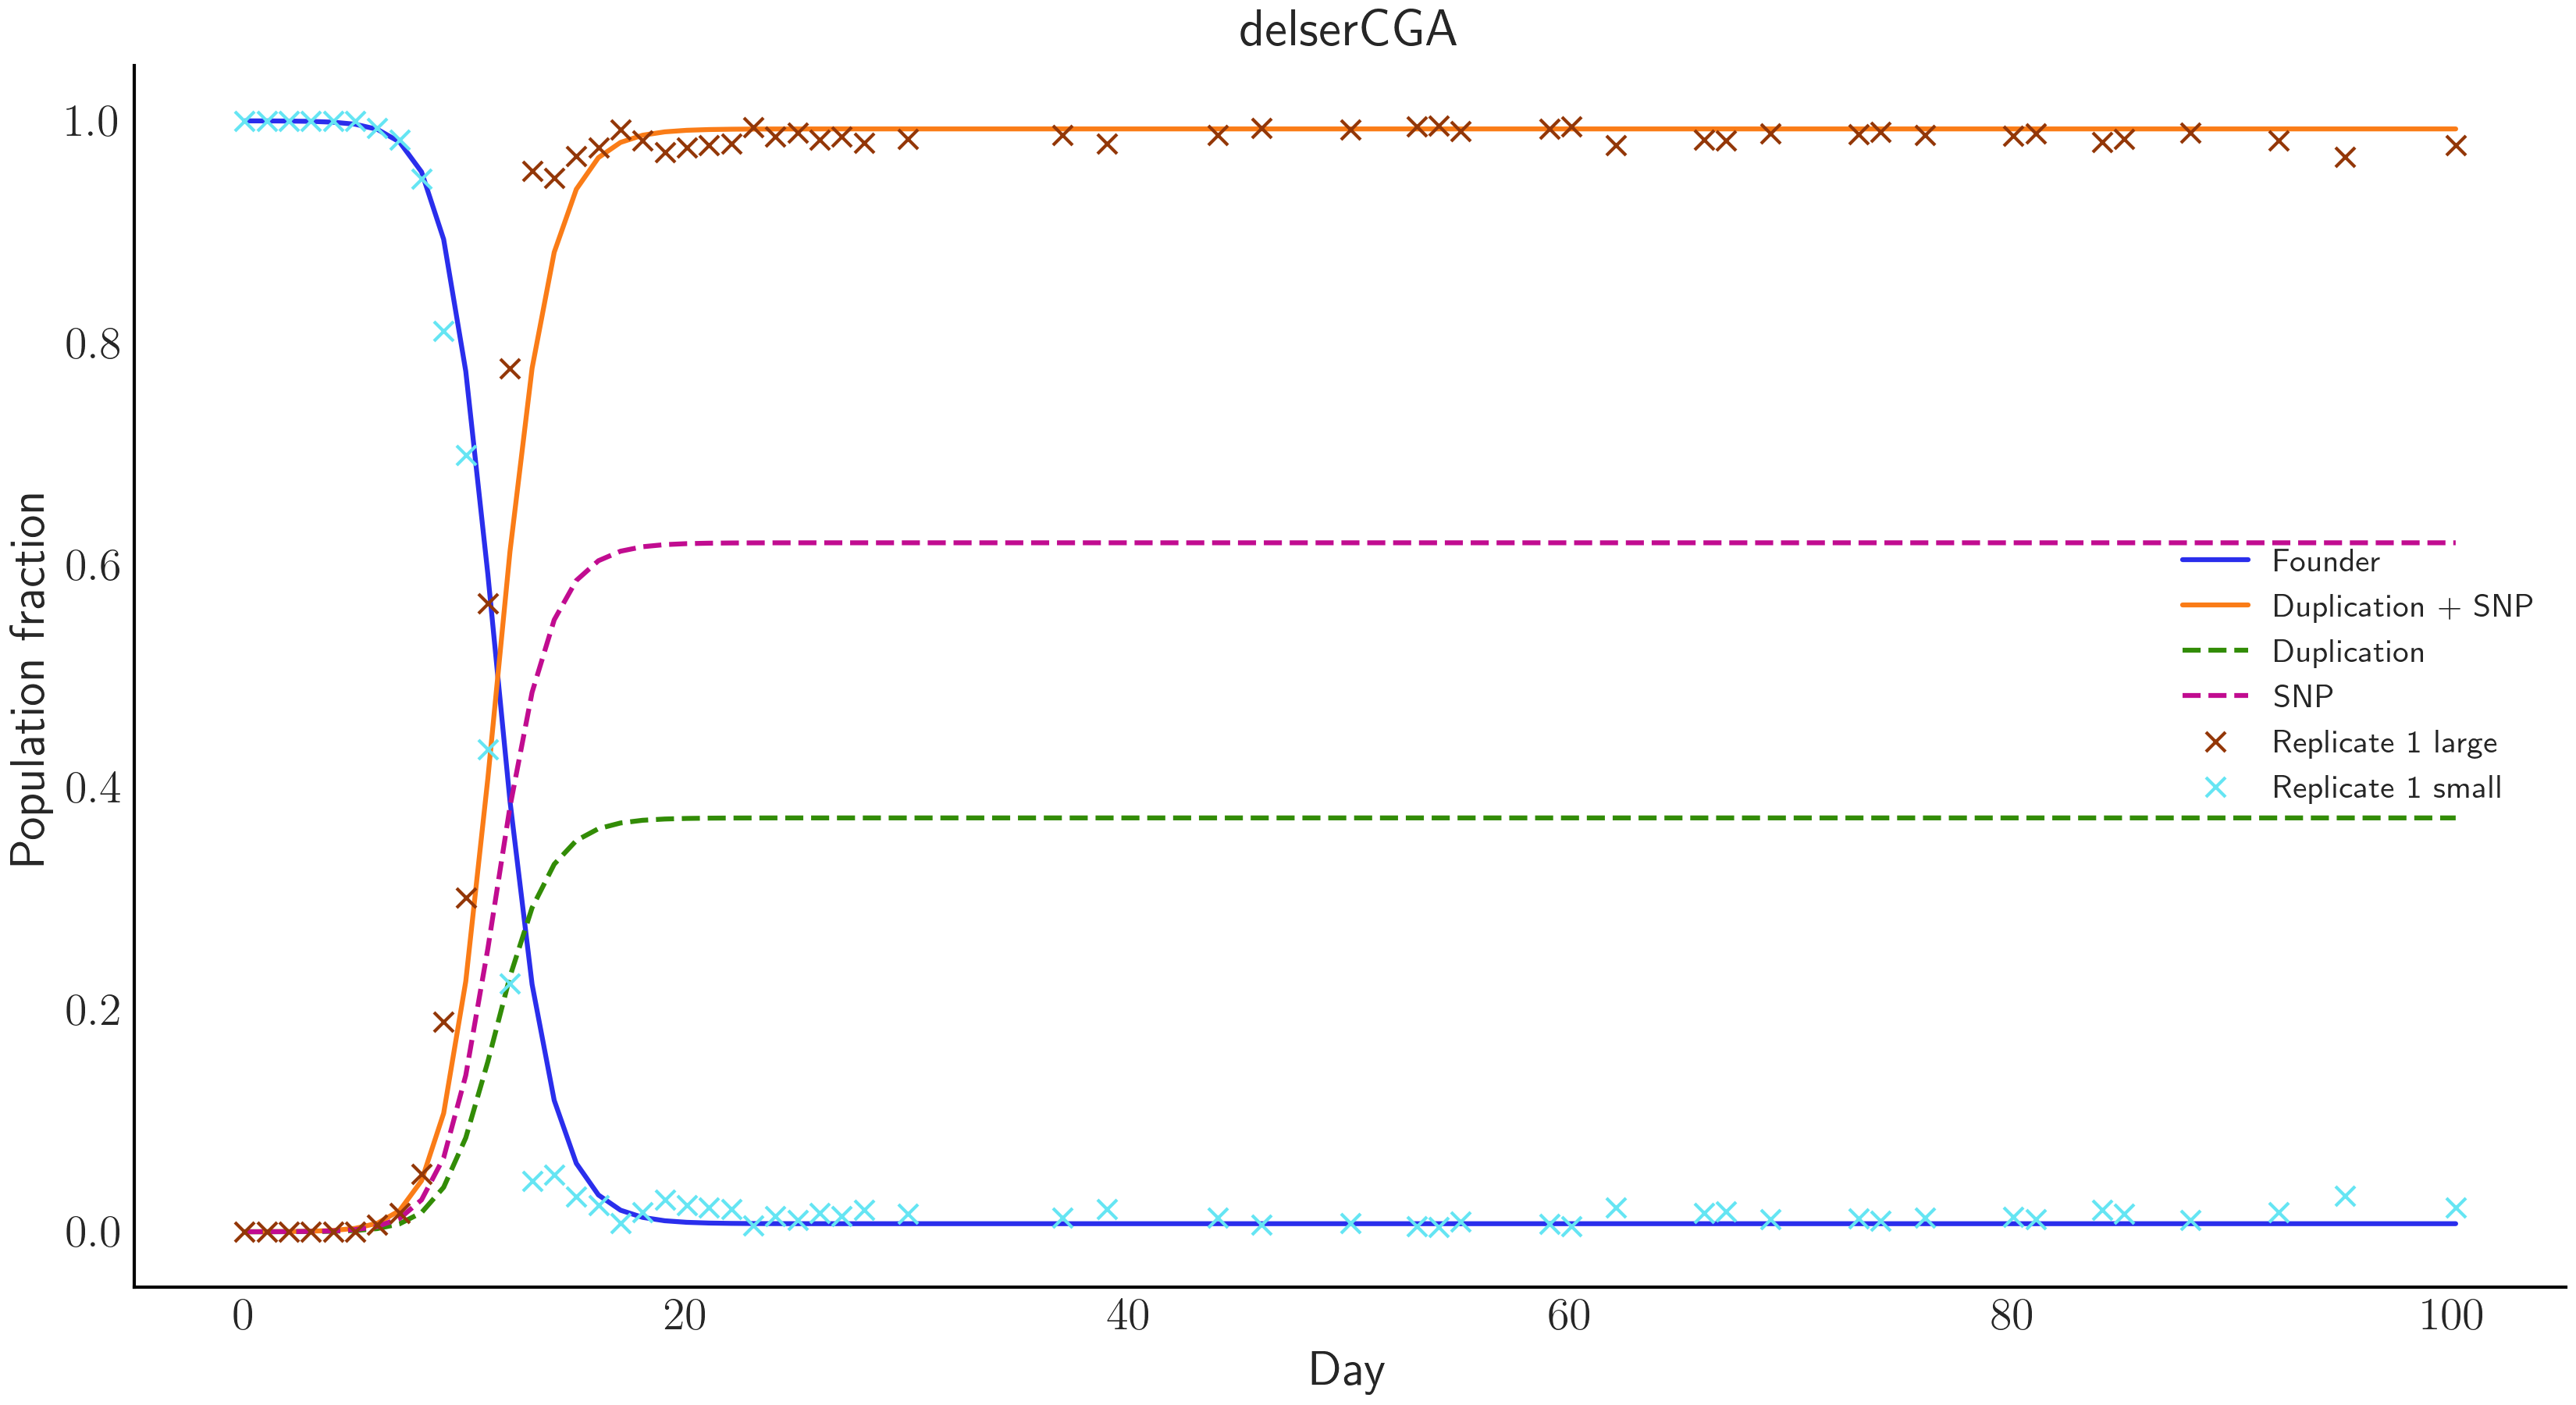
\includegraphics[width=1\linewidth]{plots/abc_3st_experiment_comparison.png}
    \caption{Sample of the experiment results using the mean of the parameters distribution}
    \label{fig:abc_3st_experiment_comparison}
\end{figure}

Furthermore, this plot shows that in the end, there is a stable equilibrium between SNP, Duplication and Founder strains with SNP being the dominant one. Moreover, this result does not completely support any of the hypotheses, perhaps signaling that it is necessary to review and update them.%To Miguel: a bit of a bold claim...

Nonetheless, these are exciting results as now we seem to be able to estimate a reasonable value for the parameters. We can use this information to impose constraints in the parameter space when carrying out calculations for the time to reach the equilibrium (see next section).

%To Miguel: to me, this fitting of the 3-state system from the data we have still does not make sense, and I am still unsure how the final proportions of SNP vs. duplication should be interpreted. I am assuming though, that these 2 proportions come from the assumption that muSF is zero?? No, muSF was not fixed to zero. We also did not have the OD for the SNP. Instead, what was done was using the same prior, but randomly choosing two different initial points for the exploration. Check that we indeed get very different final proportions when not fixing the random seed in the code.

\section{Parameter space exploration \& time to reach equilibrium}

We explore the parameter space of our models to analyze the time to reach a steady state, and the fate of the different strains, in a parameter space defined by plausible values for each parameter. We start by looking at the two state model; based on our previous work we know that the two parameters which determine the dynamics of the system are the ratio of the replication rates $(\alpha = r_M / r_F)$ and the mutation loss rate $\mu_{MF}$. Using the results of our inference task we restrict the search interval to $10^{-3} \leq \mu_{MF} \leq 2 \times 10^{-1}$ and $1 \leq \alpha \leq 2$

We say that the system has reached the steady state\footnote{The simulation ran for a maximum of 1000 days, in case that convergence was not achieved prior to that point, we show the max number of steps as the convergence time} when the variation of the population for three consecutive days is smaller than an arbitrary threshold of $\epsilon = 10^{-5}$ (see the methods section to see how convergence is defined).

\begin{figure}[H]
	\centering
	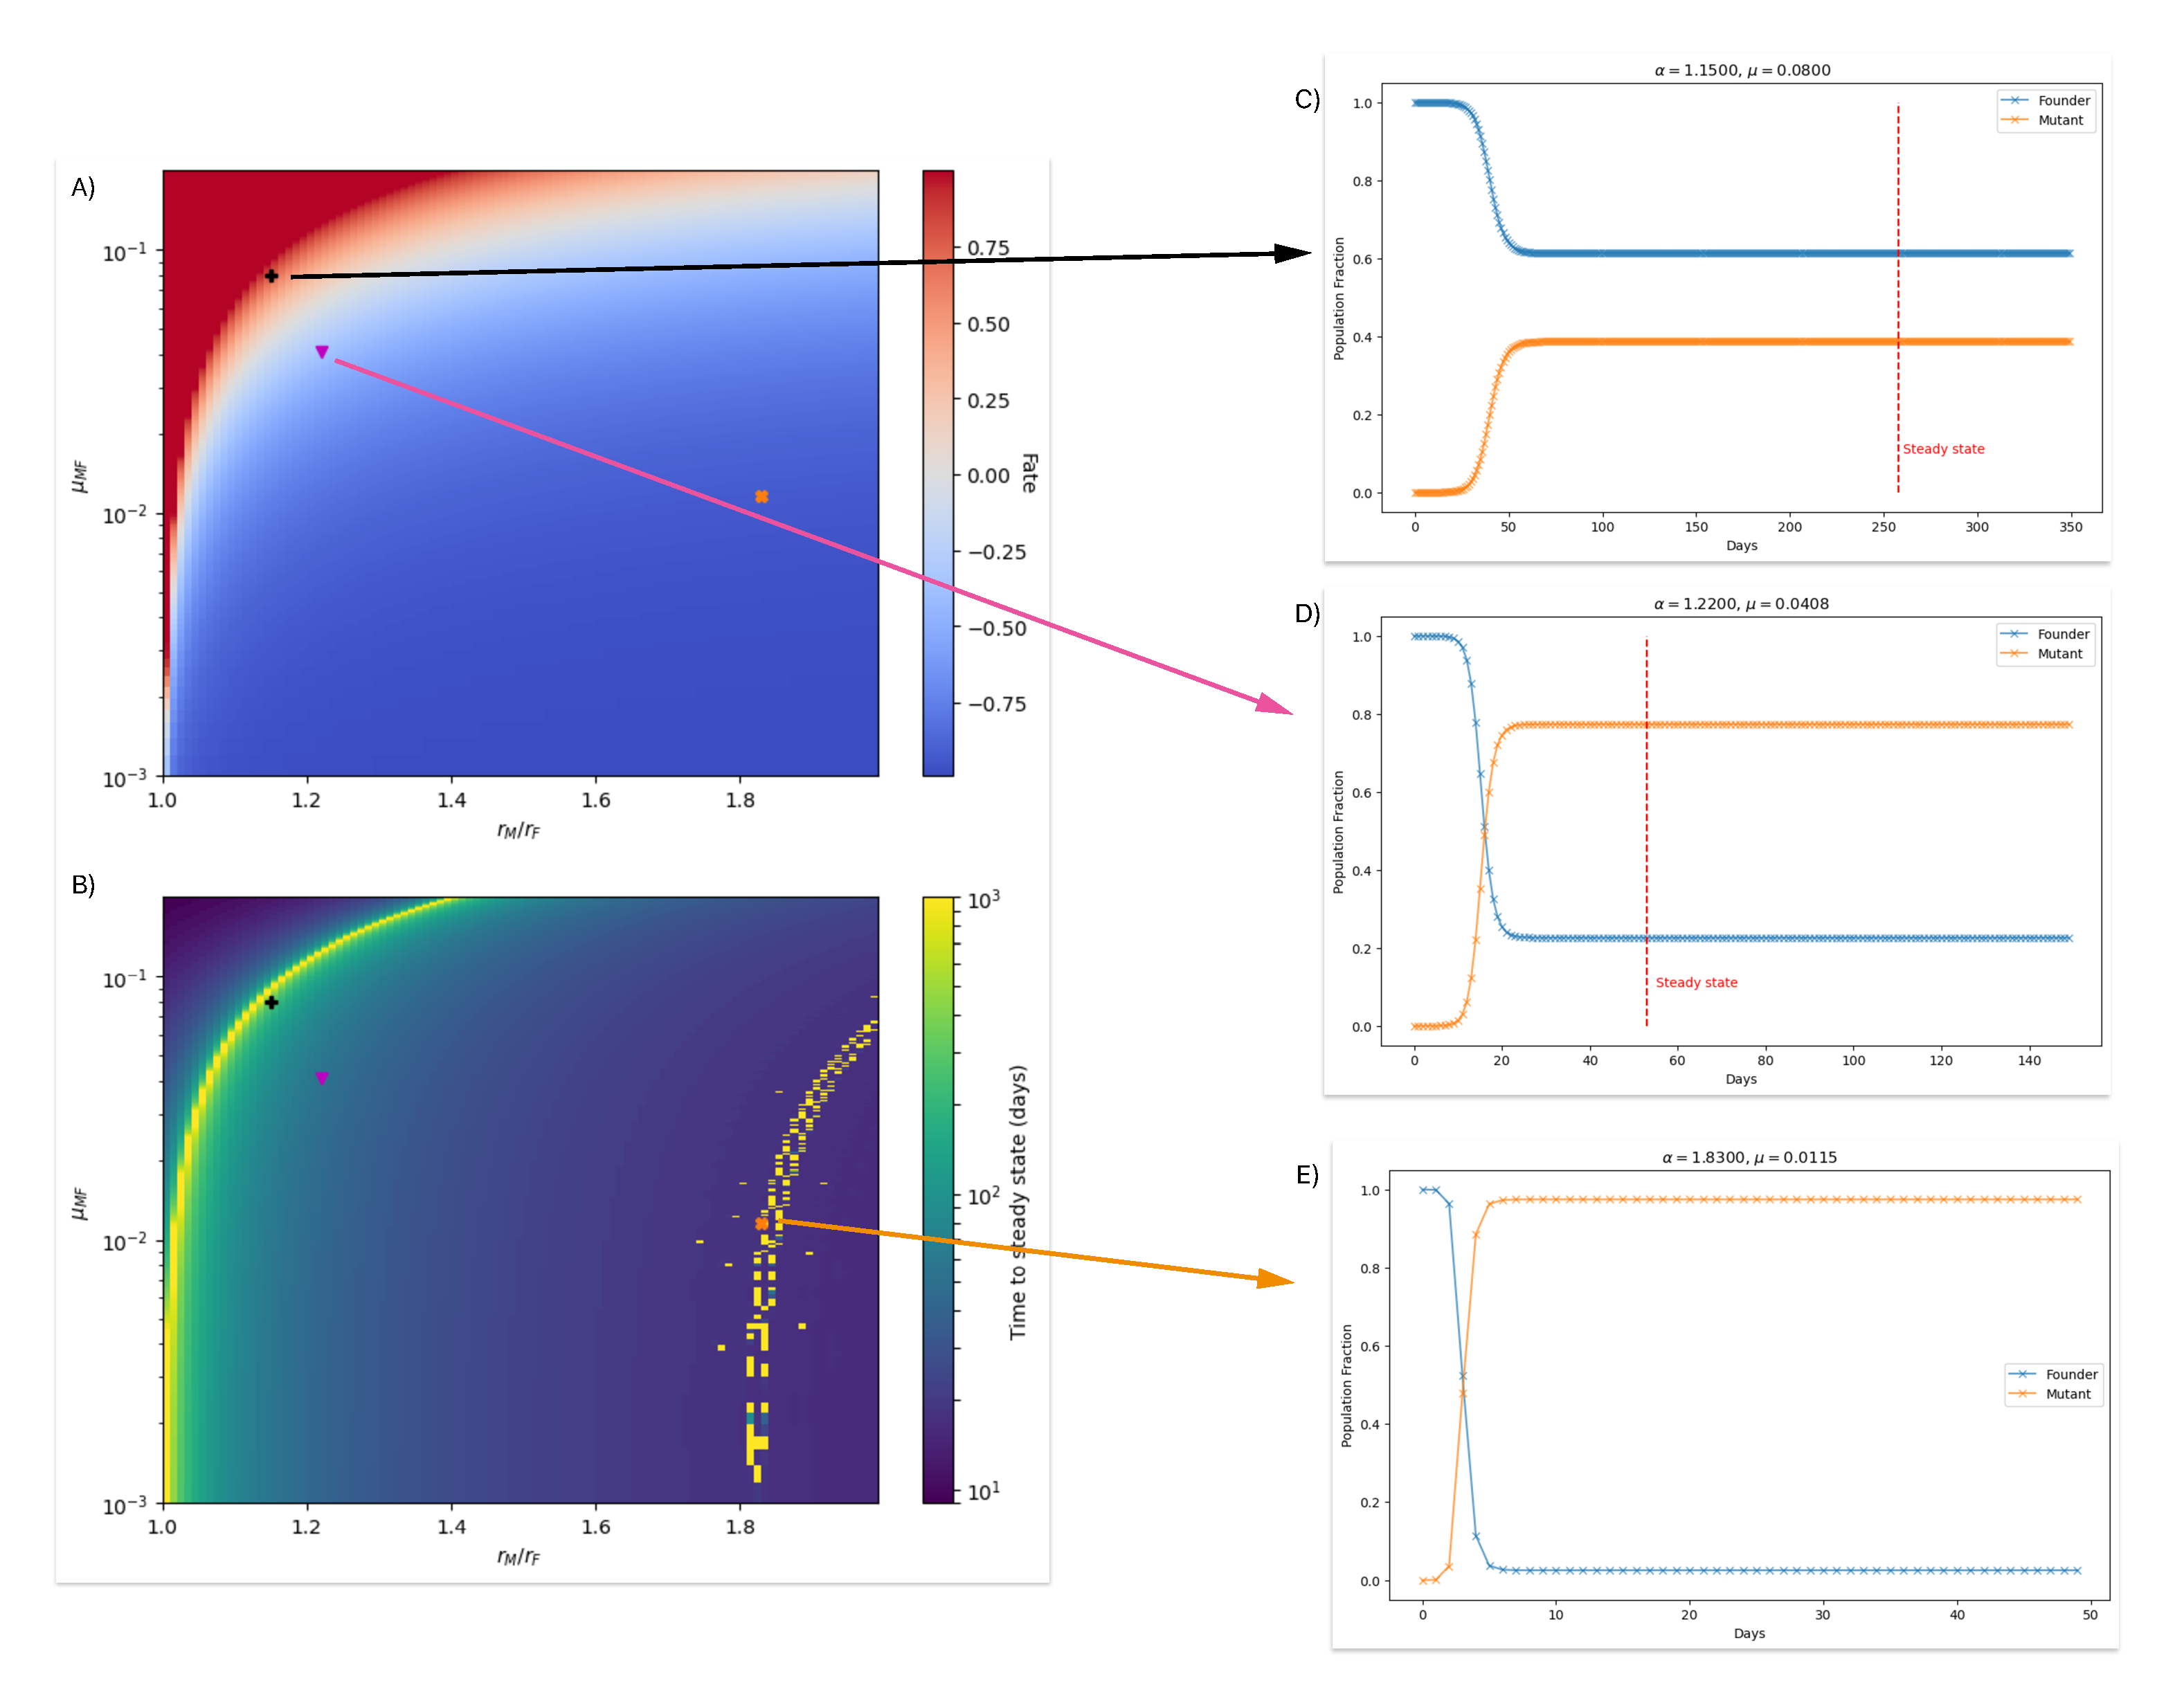
\includegraphics[scale=0.35]{big_plot_v2.pdf}
	\caption{Parameter space for the two state system. The left panel shows the difference between the bacterial abundance at the end of the experiment (top), and the time to reach the steady state (bottom). In the former, the intensity of the color indicates a higher abundance of founder (red) or mutant (blue). In the latter, the color grading represents the number of days to reach the steady state. The right panel shows the evolution of population proportions at the end of every day for areas of interest in the parameter space.}%Question for Miguel: Where is the point that corresponds to the inferred parameters? Can you explain why these 3 points are of interest? Could you show the 3 right panels with the same time scale so that it is more obvious it takes various times to converge to steady state?
	\label{fig:parameter_space_2st}
\end{figure}

The top panel in Figure \ref{fig:parameter_space_2st} displays the difference between the proportions of founder and mutant at the steady state. The red tones indicate a higher abundance of founder, whereas the blue tones higher abundance of mutants. The red areas support the intuition that a higher mutation loss rate combined with a low mutant replication rate result in a great abundance of founders, therefore there will be no coexistence of mutants and founders. %A similar affirmation is true for --> Q to Miguel: Where did that lead to?

All the lighter tones represent coexistence between founders and mutants, with a slight preference towards either population depending on the specific tone. We can see that coexistence is possible for most values of $\alpha$ but it only happens for $\mu_{MF}>10^{-2}$. %To Miguel: That is not exactly correct, is it?

In addition, we can relate the behavior in the population abundance with the time to steady state. The transition between bold and light red areas in panel A matches the yellower curve in panel B, implying that the transition between a state of coexistence to a state where the founder takes over the population causes the system to reach the steady state at a later time. %To Miguel: I did not quite get that and I'm not sure this sentence is really what you meant...

The right panel in Figure \ref{fig:parameter_space_2st} exemplifies the evolution of the population proportions for different regions of the parameter space. C and D show two points in the coexisting region.
The regions where one of the populations is dominant are characterized by small times to reach the steady state. These times get larger as we approach the regions where coexistence is possible. It is interesting to note as well, that this transition is seemingly smooth for the mutants and quite sharp for the founders.% To Miguel: I am not certain to see that amymore, with the log color plot?

%To Miguel: What I miss here, is crucial: checking that we get the same plot (top panel) if we take the analytical equilibrium of the system without saturation and bottleneck, as we suspected from the start...


%%%% Insert plot of the difference between populations

\subsection{No Bottleneck model}
In an ideal scenario, one could imagine the evolution experiment done without diluting the bacterial culture, and letting the bacterial colonies grow in the presence of infinite resources. This is clearly an experimentally impossible setting, however, implementing it into our equations provides enormous simplification to the mathematical model. A priori, we would expect to obtain the same final proportions for each strain, with the main difference between approaches being the time to reach the steady state. This time should be large for the model with a bottleneck as the carrying capacity limits the daily bacterial growth, thus delaying the convergence. This scenario is obtained by taking $K\rightarrow \infty$, then Eqs \ref{eqs:adimensional_two_state_model} become 

\begin{subequations}\label{eqs:adimensional_two_state_model_no_bottleneck}
\begin{align}
\dv{F}{\tau} &= \left(1 - \Tilde{\mu}_{FM}\right)F + \alpha \Tilde{\mu}_{MF} M \\
\dv{M}{\tau} &= \Tilde{\mu}_{FM} F + \alpha\left(1 - \Tilde{\mu}_{MF}\right)M
\end{align}
\end{subequations}

Eqs \ref{eqs:adimensional_two_state_model_no_bottleneck} have analytical solution. In the evolution experiment the initial conditions are set to $F(0) = 1, M(0) = 0$, and thus we obtained the following solution

\begin{subequations}\label{eq:solution_two_state_no_bottleneck}
\begin{align}
F(t) &= \frac{e^{\frac{a}{2}t}}{\sqrt{\Delta}}\left[  b\sinh\left(\frac{\sqrt{\Delta}}{2}t \right ) + \sqrt{\Delta}\cosh\left(\frac{\sqrt{\Delta}}{2}t \right )\right ]\\ 
C(t) &= \frac{2\mu_{FM}e^{\frac{a}{2}t}}{\sqrt{\Delta}}\sinh\left(\frac{\sqrt{\Delta}}{2}t \right )
\end{align}
\end{subequations}

Where we the constants $a, b, \Delta$ are defined as

\begin{align*}
a &= \left(1-\mu_{FM} \right ) + \alpha\left(1-\mu_{MF} \right ) \\
b &= \left(1-\mu_{FM} \right ) - \alpha\left(1-\mu_{MF} \right ) \\
\Delta &= a^2 - 4\alpha\left(1 - \mu_{FM} - \mu_{MF}\right)
\end{align*}

In this setting the population grows exponentially; however, the proportions for each strain do converge to a steady state as $t\rightarrow \infty$. This steady state is described by 

\begin{subequations}\label{eq:steady_state_no_bottleneck}
\begin{align}
f_\infty = \frac{b + \sqrt{\Delta}}{b + 2\mu_{FM} + \sqrt{\Delta}}\\
m_\infty = \frac{2\mu_{FM}}{b + 2\mu_{FM} + \sqrt{\Delta}}
\end{align}
\end{subequations}

This predictions for the proportions of the bacterial population (Figure \ref{fig:parameter_space_2st_no_bottleneck}) agree with those obtained including bottleneck effects (Figure \ref{fig:parameter_space_2st}). Here, we further expand the range of $\alpha$\footnote{Values of $\alpha < 1$ are not biologically significant, because compensatory mutations will increase the fitness of the bacteria, thus we would expect them to have a higher replication rate. However, it is useful to expand the range of $\alpha$ to gain some insight into the behaviour of the system.} 
and $\mu_{MF}$ and observe that below $\alpha = 1$ there is a sharp transition from dominance of mutants to dominance of founders, this holds for $\mu_{MF} < 10^{-3}$ 

Intuitively, we would expect that high mutation loss rates would cause the founder population to dominate the culture,

\begin{equation*}
\mu_{MF} = \frac{3\mu_{FM} - \alpha\mu_{FM} + \alpha - 1}{2\alpha}
\end{equation*}

everything above this curve are regions with 
The predictions
In Figure \ref{fig:parameter_space_2st} we observed the dominance of the founder population being determined by the value of $\mu_{MF}$; in particular, it was largely dominant for $\mu_{MF} > 10^{-2}$. Here, we expanded the plot range and observed the same behaviour. Regions with small 
Additionally, there is a sharp transition at $\alpha = 1$



\begin{figure}[H]
	\centering
	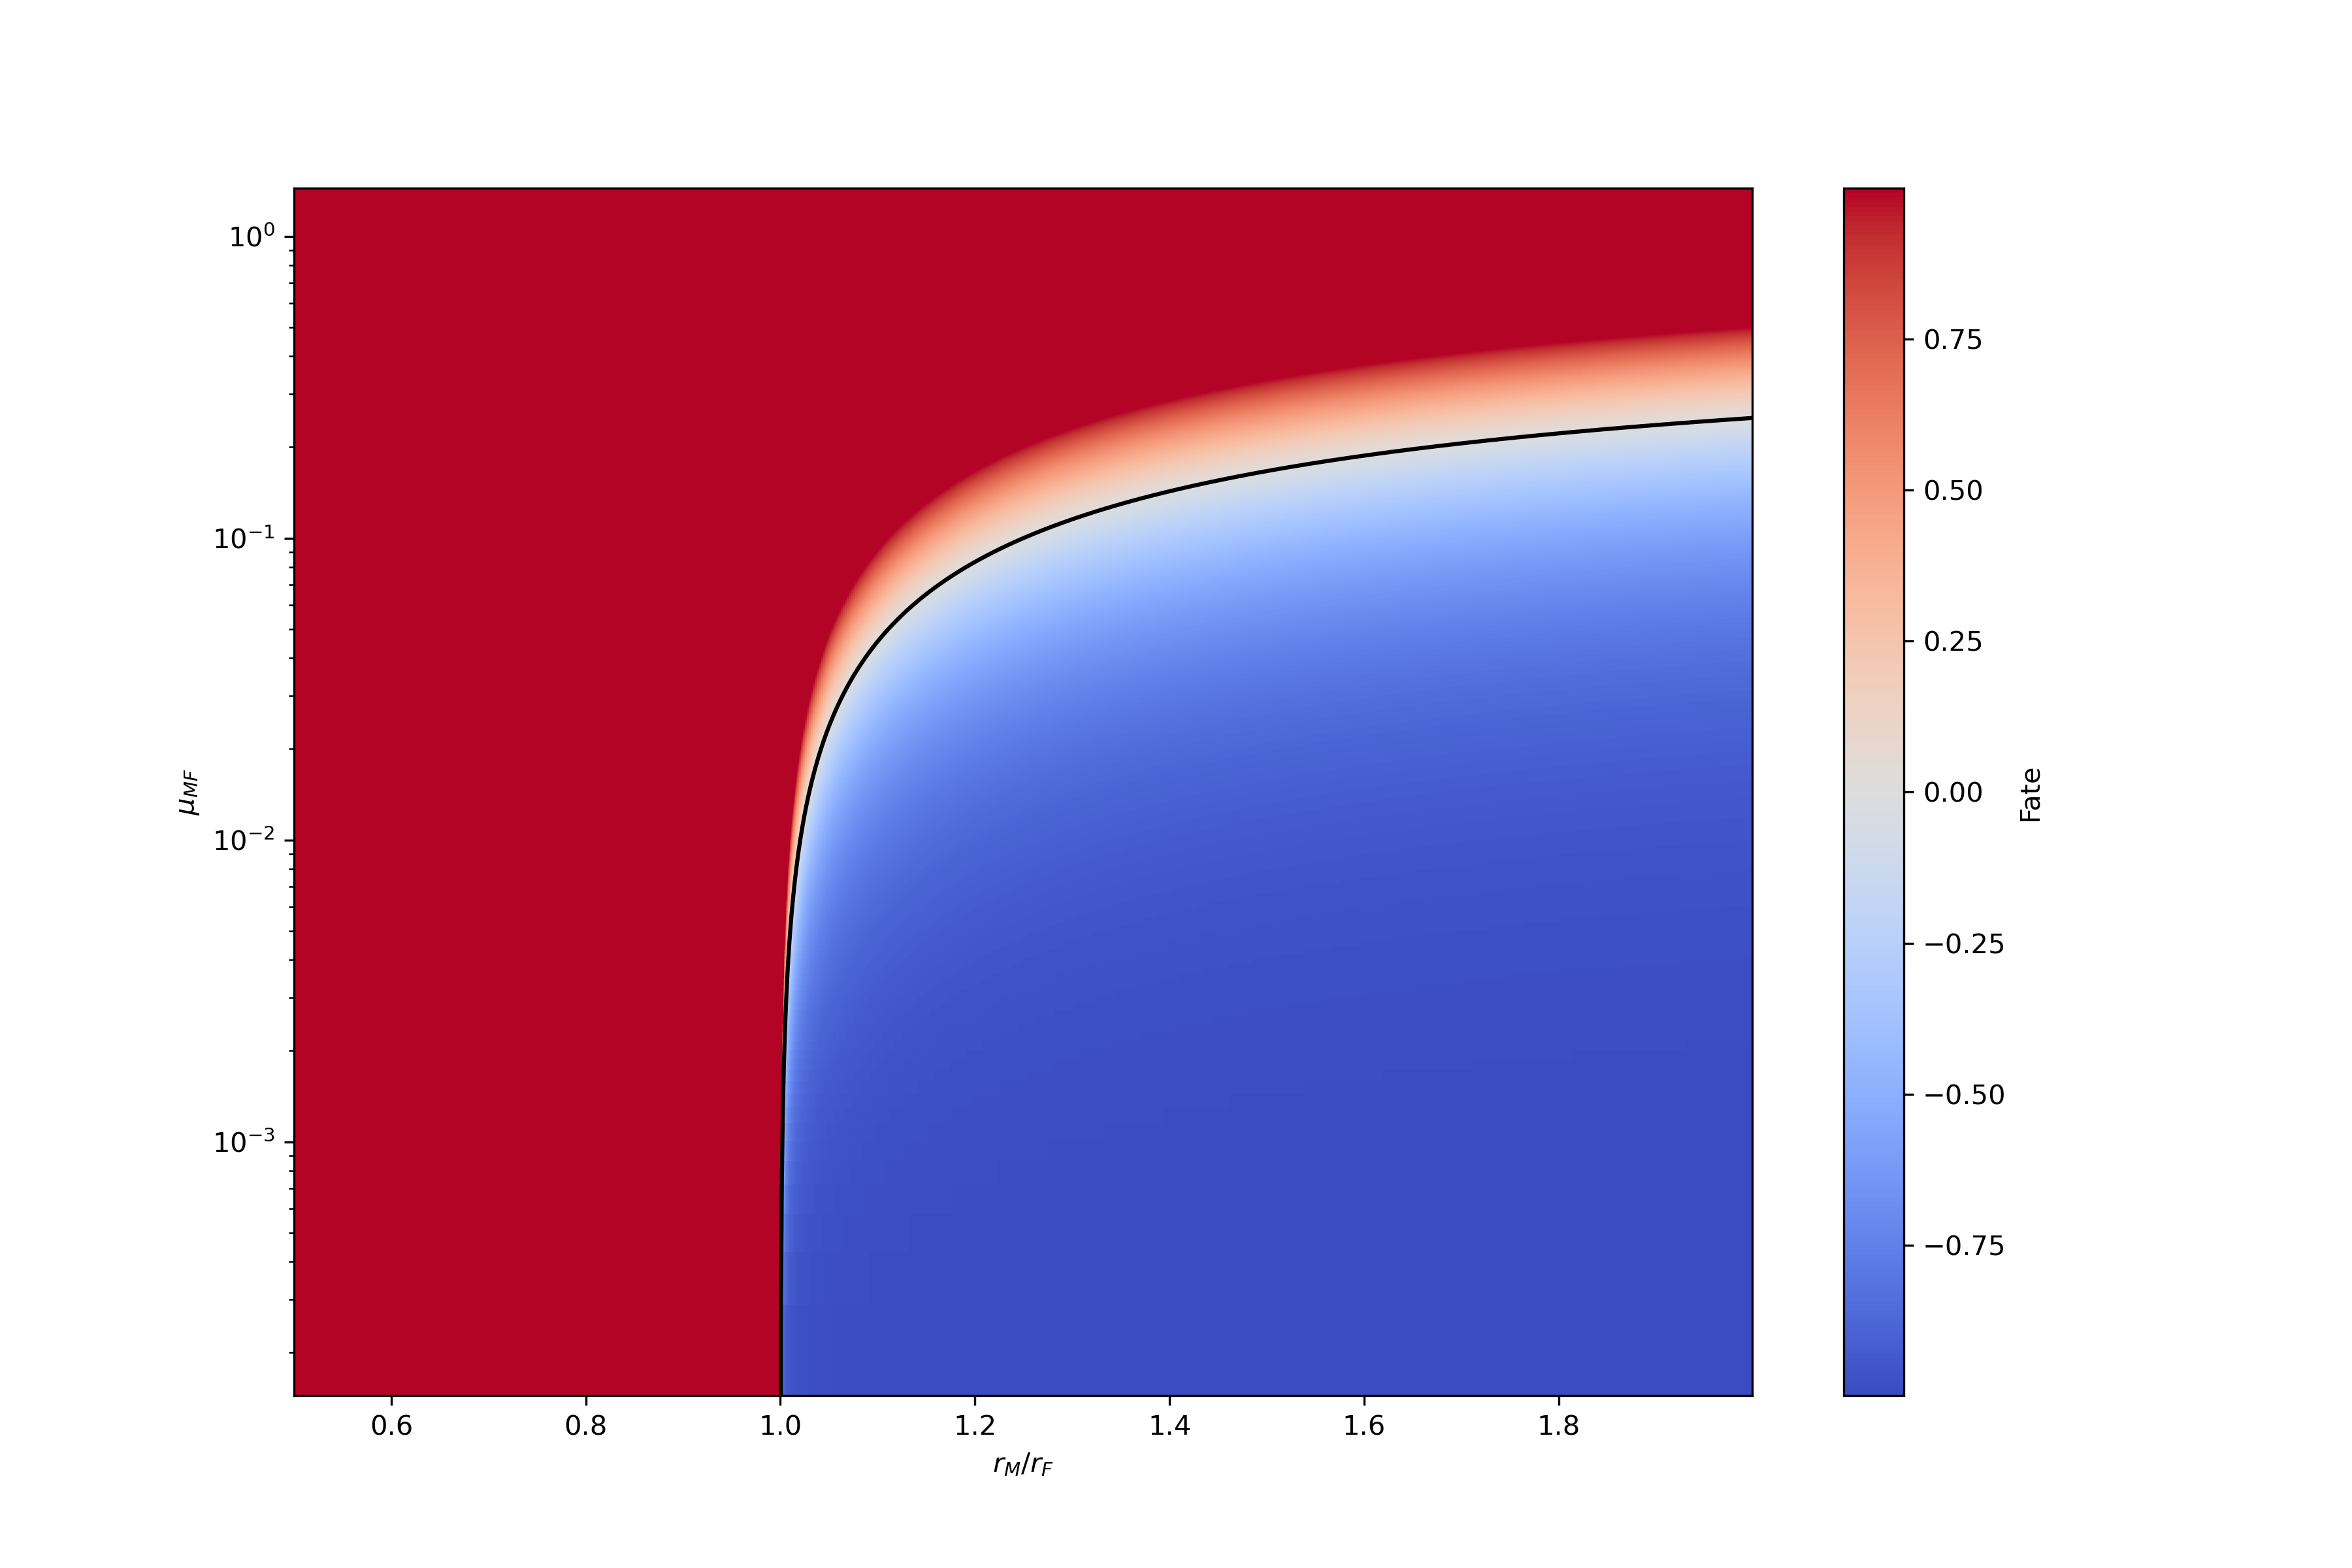
\includegraphics[scale=0.5]{plots/theoretical_fate.png}
	\caption{Theoretical prediction of the bacterial populations abundance in a two state model without bottleneck. The solid black line is the boundary between regions with more abundance of founder (red) or mutant (blue)}
	\label{fig:parameter_space_2st_no_bottleneck}
\end{figure}



\section{Perspectives}
Here I want to summarize some tasks that are still pending without any particular order
\begin{itemize}
    \item Implement a measure for the goodness of fits from the parameters obtained by Bayesian inference. So far I am only visually inspecting the results and there is no quantitative measurement of it
    \item So far I have been running all the inference algorithms for replicate 1 of the experimental data. Even though upon visual inspection all the replicates look indistinguishable, it is necessary to run the algorithms for the remaining replicates to compare the results and test the robustness of the predictions. Nonetheless, I don't expect the results to change significantly.
    \item We discussed at some point in the past weeks about the apparent symmetry of the equations. Running the experiment for the 2 state system interchanging all the parameters between Founder and Mutant will be useful to test that independence of the predictions.%I still don't think that's really needed
    \item I still need to address the time that it'll take the experiment to converge for different experimental conditions. Since so far I haven't found an analytical solution, the easiest way to do it will be to explore the parameter space using the knowledge gained from the bayesian inference results. DONE
    \item Somewhere we should explain the $ln(2)$ conversion for mutation rates. Or is that really necessary?
\end{itemize}

\ \newpage
\bibliographystyle{vancouver_modified.bst}
\bibliography{trna.bib}
%\printbibliography
\end{document}